\chapter{Studi Literatur}
\label{chapter:studi-literatur}

Bab ini akan diisi oleh studi literatur yang terkait dengan topik persoalan pada tugas akhir untuk memberikan informasi mengenai dasar teori dan literatur yang digunakan. Bab ini diharapkan dapat membantu pembaca memiliki pengetahuan yang menyeluruh dan dasar yang cukup untuk mengerti penelitian ini.

\section{Blockchain}
\label{sec:blockchain}

\subsection{Konsep dan Struktur Blockchain}
\label{subsec:konsep-struktur-blockchain}

Blockchain adalah sebuah sistem pencatatan data terdistribusi yang tersusun atas serangkaian blok, di mana setiap blok menyimpan daftar transaksi secara lengkap seperti \textit{public ledger} konvensional. Data disimpan secara terdistribusi pada banyak \textit{node} dalam jaringan, sehingga tidak ada entitas terpusat yang mengontrol keseluruhan sistem. Setiap blok yang memuat transaksi harus divalidasi menggunakan mekanisme konsesus tertentu sebelum ditambahkan ke dalam rantai blok. Proses konsensus melibatkan mayoritas dari \textit{node} untuk menyetujui atau menolak \textit{state} baru dari \textit{ledger}, sehingga menjamin integritas dan keaslian dari data \parencite{zheng2018blockchain,nofer2017blockchain}.

Pada sistem Blockchain klasik, setiap blok umumnya memiliki daftar transaksi yang lengkap, ditambah dengan \textit{timestamp} pembuatan blok, nilai \textit{hash} dari blok sebelumnya ("\textit{parent}"), dan sebuah \textit{nonce}, yang adalah sebuah angka acak yang digunakan untuk mekanisme verifikasi \textit{hash}. 
Konsep ini memastikan integritas dari Blockchain dimulai dari blok pertama ("\textit{genesis block}") sampai ke blok terakhir yang akan terus bertambah, karena setiap perubahan data akan membuat nilai \textit{hash} dari sebuah blok berubah, yang harus dipropagasikan ke setiap blok setelahnya.

Aspek penting dari sebuah Blockchain adalah proses konsensus yang dimilikinya, yang dilakukan dengan mengikuti sebuah kumpulan aturan dan prosedur untuk mempertahankan himpunan fakta yang koheren diantara beberapa \textit{participating nodes}. Terdapat banyak mekanisme konsensus yang berbeda yang digunakan dalam \textit{Blockchain network} yang berbeda. Dalam kasus \textit{Bitcoin}, \textit{ledger} yang dianggap \textit{ledger} yang \textit{valid} adalah \textit{ledger} dengan \textit{chain} terpanjang (\textit{longest chain}) \parencite{swanson2015consensus}.

\begin{figure}[ht]
	\centering
	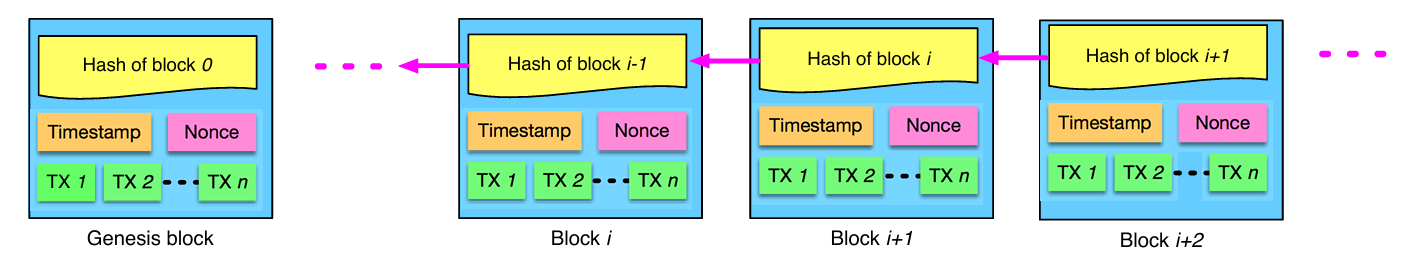
\includegraphics[width=1\textwidth]{resources/chapter-2/struktur-blockchain.png}
	\caption{Struktur blok di dalam Blockchain \parencite{zheng2018blockchain}}
	\label{image:struktur-blockchain}
\end{figure}

Struktur klasik dari sebuah blok pada Blockchain terdiri dari \textit{block header} dan \textit{block body} seperti pada Gambar \ref{image:struktur-blok}. Secara spesifik, \textit{block header} terdiri dari:

\begin{enumerate}
	\item \textit{Block Version}: mengindikasikan set dari aturan validasi yang diikuti.
	\item \textit{Parent Block Hash}: 256-bit \textit{hash} dari blok sebelumnya.
	\item \textit{Merkle Tree Root}: hasil \textit{hash} dari seluruh transaksi pada blok menggunakan mekanisme \textit{Merkle Tree}.
	\item \textit{Timestamp}: \textit{timestamp} saat ini dalam detik sejak 1970-01-01T00:00 UTC.
	\item \textit{nBits}: target \textit{hash} saat ini dalam format \textit{compact}.
	\item \textit{nonce}: \textit{number used only once}, sebuah angka yang digunakan untuk menambahkan tingkat keacakan dari nilai \textit{hash}.
\end{enumerate}

\begin{figure}[ht]
	\centering
	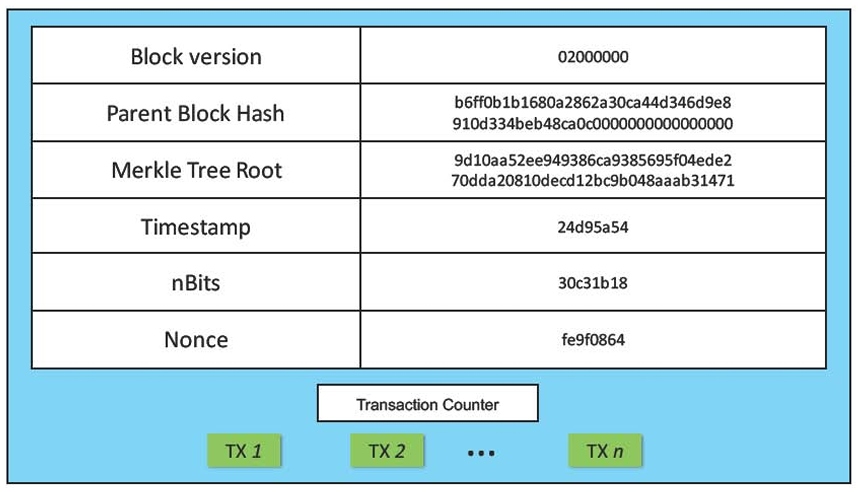
\includegraphics[width=0.7\textwidth]{resources/chapter-2/struktur-block.png}
	\caption{Struktur blok \parencite{zheng2018blockchain}}
	\label{image:struktur-blok}
\end{figure}

\subsection{Karakteristik Blockchain}
\label{subsec:karakteristik-blockchain}

Implementasi dari Blockchain memunculkan karakteristik dari Blockchain itu sendiri. Karakteristik ini dapat muncul secara inheren dari sistem dasar di mana Blockchain dibangun, ataupun muncul karena implementasi spesifik Blockchain. Beberapa karakteristik penting Blockchain \parencite{aimar2023extraction}:

\begin{itemize}
	\item \textit{Decentralized}: Tidak ada sebuah entitas terpusat yang mengontrol jaringan. Seluruh \textit{participants} mengikuti protokol yang berlaku dan memiliki kontrol yang sama.
	\item \textit{Distributed}: Komputasi dilakukan pada sejumlah \textit{node} atau komputer yang berbeda, yang tersebar dan saling berinteraksi melalui sebuah \textit{p2p network}. Kegagalan sebuah mesin seharusnya tidak mengganggu jalannya protokol.
	\item \textit{Immutable}: Tidak memungkinkan untuk mengubah \textit{history} apapun yang sudah tertulis di dalam Blockchain. Setelah sebuah blok divalidasi dan dimasukkan ke dalam Blockchain, tidak dapat dimodifikasi.
	\item \textit{Autonomous}: Blockchain berjalan secara otomatis tanpa perlu campur tangan dari pihak ketiga. Setiap transaksi akan dieksekusi sesuai dengan aturan yang sudah ditentukan.
	      % \item \textit{Permissionless}: Semua orang dapat secara aktif berpartisipasi di dalam semua \textit{role} di dalam jaringan tanpa perlu meminta \textit{permission}.
	      % \item \textit{Permissioned}: Mewajibkan seluruh aktor di dalam jaringan mendapatkan \textit{authorization} secara eksplisit.
	\item \textit{Transparent}: Semua orang dapat secara independen melihat dan mengunduh data dari Blockchain.
	\item \textit{Pseudoanonymous}: \textit{Participants} dalam sebuah \textit{Blockchain network} tidak perlu membuktikan identitas asli mereka. Seluruh aktivitas di dalam jaringan akan disambungkan ke sebuah \textit{address}, bukan identitas asli seseorang.
	      % \item \textit{Account-based}: data disimpan berdasarkan akun, dan setiap akun memiliki \textit{balance} yang dapat digunakan. Kepemilikan sebuah akun dibuktikan dengan kepemilikan \textit{private key} untuk akun tersebut.
	      % \item \textit{UTXO-based}: Selain \textit{account-based}, model \textit{UTXO} hanya memiliki konsep dari transaksi. \textit{User} harus membuktikan bahwa mereka memiliki \textit{private key} untuk membuka kunci dari sebuah hasil transaksi untuk menggunakan \textit{balance} yang dimiliki. \textit{Balance} dari seorang \textit{user} adalah penjumlahan seluruh nilai dari hasil transaksi yang dapat dibuka dan digunakan.
\end{itemize}

\subsection{Off-Chain}
\label{subsec:offchain}

Off-chain adalah sebuah proses atau transaksi yang dilakukan di luar jaringan Blockchain utama. Dalam konteks Lightning Network, transaksi off-chain dilakukan di dalam sebuah \textit{payment channel}, di mana beberapa transaksi dapat berlangsung antara dua atau lebih pihak tanpa harus langsung direkam pada Blockchain. Proses ini memungkinkan para pihak untuk saling bertransaksi secara cepat dan dengan biaya yang jauh lebih rendah karena tidak memerlukan konfirmasi untuk setiap transaksi di jaringan utama.

Hanya saat \textit{payment channel} ditutup, transaksi-transaksi off-chain tersebut akan diselesaikan secara \textit{final} dengan melakukan \textit{settling} pada Blockchain. Mekanisme ini memastikan bahwa keamanan dan integritas data tetap terjaga karena hasil akhir dari semua transaksi off-chain dicatat secara permanen di Blockchain melalui proses konsensus. Selain itu, transaksi off-chain umumnya dilakukan menggunakan protokol Layer 2, seperti Payment Channels, Sidechains, dan Rollups \parencite{sguanci2021layer}. Pendekatan ini tidak hanya mengurangi beban jaringan utama, tetapi juga memungkinkan terjadinya \textit{micropayments} dan peningkatan \textit{throughput} jaringan secara signifikan.

Berikut merupakan beberapa keuntungan dari transaksi off-chain:

\begin{enumerate}
	\item \textbf{Efisiensi dan Skalabilitas} \newline
	      Transaksi off-chain memungkinkan jaringan Blockchain untuk menangani lebih banyak transaksi tanpa mengorbankan kecepatan dan efisiensi Blockchain.
	\item \textbf{Privasi} \newline
	      Transaksi off-chain tidak langsung tercatat di Blockchain, sehingga memungkinkan para pengguna untuk menjaga privasi mereka.
	\item \textbf{Pengurangan Biaya} \newline
	      Transaksi off-chain biasanya memiliki biaya yang lebih rendah dibandingkan dengan transaksi on-chain karena hanya perlu transaksi untuk pembukaan dan penutupan \textit{channel}.
	\item \textbf{Interoperabilitas} \newline
	      Protokol Layer 2 memungkinkan jaringan Blockchain yang berbeda untuk berinteraksi satu sama lain, sehingga memperluas kemungkinan penggunaan dan penerapan teknologi Blockchain.
\end{enumerate}


\newpage
\section{Ethereum}
\label{sec:ethereum}

% \subsection{Sejarah dan Pengembangan Ethereum}
\label{subsec:sejarah-pengembangan-ethereum}


Ethereum adalah sebuah \textit{platform} berbasis Blockchain yang berfokus pada pembangunan aplikasi terdesentralisasi dan Smart Contracts, dengan serangkaian \textit{tradeoffs} yang berbeda. 
Dikembangkan oleh Vitalik Buterin pada tahun 2015, Ethereum memperluas konsep dasar Blockchain yang sebelumnya hanya terbatas untuk transaksi. Ethereum melakukannya dengan membangun sebuah \textit{layer} fondasi dalam bentuk sebuah Blockchain dengan \textit{built-in Turing-complete programming language}, yaitu Solidity, yang memungkinkan pengembang untuk membangun aplikasi terdesentralisasi yang kompleks dan Smart Contracts yang menjalankan logika dan sistem di dalam Blockchain \parencite{buterin2013ethereum}. 

Secara teknis, perbedaan utama Ethereum dengan Bitcoin adalah perbedaan dari jenis data yang disimpan di dalam Blockchain. Bitcoin hanya menyimpan data kepemilikan mata uang, sedangkan Ethereum menyimpan \textit{state transitions} dari \textit{data store} yang lebih umum. Ethereum memiliki \textit{memory} yang dapat menyimpan data dan kode, dan Blockchain Ethereum dapat digunakan untuk melacak bagaimana perubahan dari \textit{memory} dari waktu ke waktu. Seperti layaknya \textit{general-purpose computers}, Ethereum dapat menjalankan kode ke dalam \textit{state machine} yang dimilikinya, dan menyimpan hasilnya ke dalam Blockchain. Perbedaan utama Ethereum dengan kebanyakan \textit{general-purpose computers} adalah mekanisme perubahan \textit{state} di dalam Ethereum yang diatur oleh rangkaian aturan di dalam konsensus, dan distribusi global dari \textit{state} \parencite{antonopoulos2018mastering}.


% Bahasa pemrograman bawaan Ethereum yang \textit{Turing-complete} adalah Solidity, yang digunakan untuk menulis Smart Contracts di Ethereum. 
% Solidity adalah bahasa dengan paradigma berorientasi objek, seluruh program Smart Contract akan dikompilasi menjadi sebuah \textit{Bytecode}, dalam kasus ini menjadi bentuk EVM Bytecode, dan spesifikasinya dituliskan pada sebuah Application Binary Interface (ABI). Dengan bahasa pemrograman yang \textit{Turing-complete} dan mekanisme eksekusi yang terjamin dengan EVM, Ethereum memberikan kemampuan bagi pengembang untuk mengembangkan sebuah aplikasi yang terdesentralisasi, yang disebut juga sebagai \textit{dApps}, di mana kode dan data disimpan di dalam Blockchain, sehingga mendapatkan karakteristik bawaan dari karakteristik Blockchain \parencite{buterin2013ethereum}.

% , dengan menambahkan sebuah bahasa pemrograman \textit{Turing-complete} untuk mengembangkan Smart Contracts yang menjalankan logika dan sistem di dalam Blockchain. Ethereum melakukannya dengan membangun sebuah fondasi 



\subsection{Ethereum Virtual Machine dan Smart Contracts}
\label{subsec:evm-smart-contract}

Ethereum Virtual Machine (EVM) adalah sebuah mesin komputasi yang serupa dengan mesin virtual lainnya seperti Java Virtual Machine (JVM) atau .NET Common Language Runtime (CLR). EVM adalah mesin \textit{Turing-complete}, yang berarti bahwa EVM dapat menjalankan kode apapun yang diberikan kepadanya, dengan batasan waktu dan biaya, yang dihitung dengan \textit{gas}. EVM menjalankan kode yang ditulis dalam bahasa pemrograman Solidity, yang kemudian dikompilasi menjadi EVM Bytecode, yang kemudian dijalankan di dalam EVM. EVM memiliki beberapa komponen, seperti \textit{world state}, \textit{storage}, \textit{memory}, \textit{stack}, dan \textit{program counter} yang saling berinteraksi untuk mengeksekusi Smart Contract Bytecode seperti pada gambar \ref{image:evm-architecture} \parencite{wood2014ethereum}.

\textit{Gas} adalah unit yang digunakan untuk mengukur biaya komputasi dan penyimpanan yang digunakan untuk menjalankan aksi di dalam Blockchain Ethereum. \textit{Gas} adalah komponen penting dalam Ethereum dan menjalankan peran sebagai \textit{buffer} antara harga dari Ethereum dan \textit{reward} untuk \textit{miner} dan sebagai pertahanan untuk serangan \textit{denial-of-service attacks}.

\begin{figure}[ht]
	\centering
	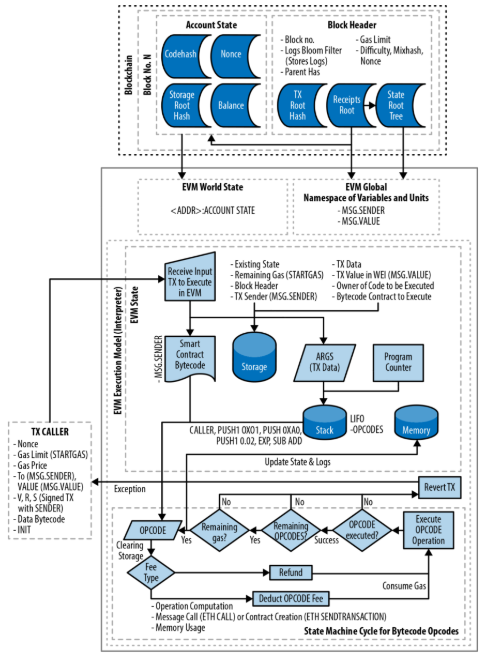
\includegraphics[width=0.7\textwidth]{resources/chapter-2/evm-architecture.png}
	\caption{Arsitektur EVM \parencite{antonopoulos2018mastering}}
	\label{image:evm-architecture}
\end{figure}

Smart Contracts adalah program yang ditulis untuk berjalan di atas Blockchain Ethereum. Smart Contracts adalah kode yang berjalan di dalam EVM, yang memungkinkan pengguna untuk membuat aturan dan logika yang akan dieksekusi secara otomatis ketika kondisi tertentu terpenuhi. 
% Berikut adalah alur dari eksekusi Smart Contracts di dalam EVM:

% \begin{enumerate}
% 	\item \textbf{Inisiasi Transaksi} \newline
% 	      Eksekusi dimulai saat ada transaksi yang memanggil fungsi pada Smart Contract yang mencakup data input, alamat Smart Contract, dan jumlah \textit{gas} yang dialokasikan.
% 	\item \textbf{Propagasi dan Validasi Transakksi} \newline
% 	      Transaksi akan dipropagasikan ke seluruh jaringan dan menunggu validasi awal untuk memastikan transaksi memenuhi kriteria.
% 	\item \textbf{Mempool dan Pemilihan oleh Validator} \newline
% 	      Transaksi yang telah diverifikasi akan dimasukkan ke dalam \textit{mempool}, yaitu \textit{queue} transaksi yang menunggu untuk dimasukkan ke dalam blok oleh validator (\textit{miner} dalam konsensus PoS).
% 	\item \textbf{Pembuatan dan Validasi Block} \newline
% 	      Transaksi yang terpilih akan disusun ke dalam sebuah blok yang kemudian divalidasi melalui mekanisme konsensus.
% 	\item \textbf{Eksekusi di EVM} \newline
% 	      Blok yang telah divalidasi akan ditambahkan ke dalam blockchain, dan setiap transaksi di dalam blok tersebut akan dieksekusi oleh EVM. Proses eksekusinya dimulai dari kompilasi Smart Contract dalam Solidity menjadi Bytecode, lalu instruksi Bytecode akan dijalankan sesuai dengan biaya \textit{gas} yang dialokasikan, dan hasilnya akan disimpan secara permanan di dalam blockchain.
% 	\item \textbf{Finalisasi dan Pencatatan di Blockchain} \newline
% 	      Hasil dari eksekusi Smart Contract akan dicatat di dalam blockchain dan menjadi \textit{state} baru pada blockchain.
% \end{enumerate}

% Ethereum Virtual Machine (EVM) adalah sebuah lingkungan eksekusi untuk Smart Contracts di Ethereum, yang memungkinkan kode berjalan di seluruh jaringan Ethereum secara terdistribusi. EVM adalah sebuah mesin \textit{Turing-complete}, yang berarti bahwa EVM dapat menjalankan kode apapun yang diberikan kepadanya, dengan batasan waktu dan biaya yang ditentukan oleh \textit{gas} \parencite{wood2014ethereum}. EVM menjalankan kode yang ditulis dalam bahasa pemrograman Solidity, yang kemudian dikompilasi menjadi EVM Bytecode, yang kemudian dijalankan di dalam EVM. EVM memiliki beberapa karakteristik, seperti \textit{state}, \textit{storage}, \textit{memory}, \textit{stack}, dan \textit{program counter} \parencite{wood2014ethereum}.

% \subsection{ABI}
\label{subsec:abi}

\begin{figure}[ht]
	\centering
	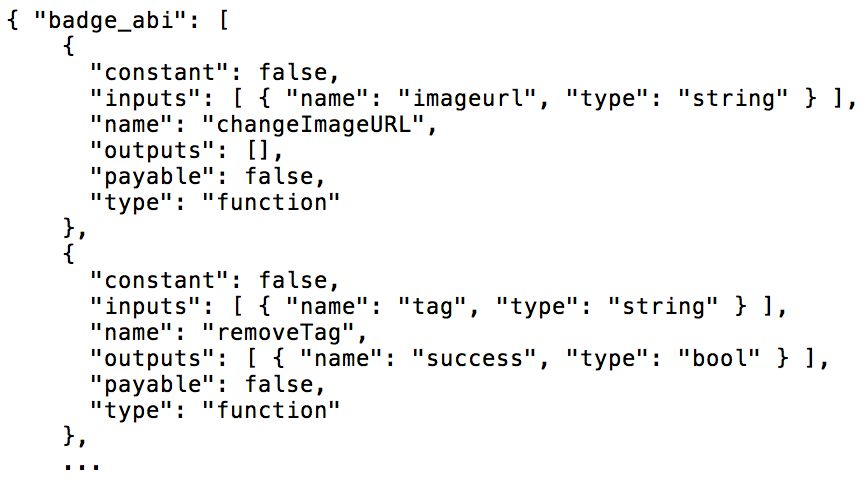
\includegraphics[width=0.7\textwidth]{resources/chapter-2/smart-contract-abi.jpg}
	\caption{Contoh ABI dari sebuah Smart Contract \parencite{third2017linked}}
	\label{image:abi-example}
\end{figure}

Application Binary Interface (ABI) adalah sebuah konvensi yang mendefinisikan aspek-aspek kode yang dihasilkan selama kompilasi, seperti representasi data, penggunaan \textit{register}, dan konvensi pemanggilan fungsi \parencite{sciencedirect2024}. Dalam konteks Smart Contracts yang ditulis dengan bahasa Solidity dan dikompilasi, hasil dari kompilasinya akan berbentuk EVM Bytecode untuk dieksekusi di dalam EVM, disertai dengan ABI yang mendefinisikan Smart Contract tersebut, seperti pada gambar \ref{image:abi-example}.

\subsection{Decentralized Applications (dApps)}
\label{subsec:dapps}

Decentralized Applications (dApps) adalah sebuah aplikasi yang berjalan di atas infrastruktur blockchain dengan memanfaatkan Smart Contracts untuk menyediakan fungsionalitasnya. Karena dApps berjalan di atas blockchain, dApps mewarisi sifat-sifat yang inheren dari blockchain, seperti terdesentralisasi, \textit{immutable}, transparan, dan sifat-sifat lainnya \parencite{investopedia2024}. dApps tidak berbeda dari aplikasi tradisional dari sisi pengguna, perbedaannya hanya terletak pada komputasi dari fungsionalitas yang diberikan oleh dApps dilakukan menggunakan Smart Contracts dan seluruh datanya terletak di dalam blockchain \parencite{metcalfe2020ethereum}.



\subsection{Etherscan}
\label{subsec:etherscan}

Etherscan adalah sebuah \textit{block explorer}, \textit{search engine} untuk pengguna agar dapat dengan mudah melihat, mengonfirmasi, dan memvalidasi transaksi untuk Blockchain Ethereum. Etherscan didirikan oleh Matthew Tan pada tahun 2015, dan berdiri secara independen dari Ethereum Foundation. Etherscan melakukan \textit{indexing} terhadap Blockchain untuk menampilkan informasinya, di mana informasi tersebut digunakan untuk menyediakan API untuk pengembang mengintegrasikan informasi Blockchain Ethereum ke dalam aplikasinya \parencite{etherscan2024}.

\subsection{Standard Smart Contract}
\label{subsec:standard-sc}

Smart Contract Standards adalah kumpulan pedoman dan spesifikasi yang perlu diikuti oleh sebuah Smart Contracts agar dapat beroperasi secara konsisten dan kompatibel di seluruh jaringan. Di dalam Ethereum, standar tersebut didefinisikan dalam bentuk Ethereum Request for Comments (ERC), yang merupakan seperangkat standar teknis yang digunakan untuk mengatur cara pengembangan Smart Contract. ERC diperkenalkan oleh Fabian Vogelsteller dan Vitalik Buterin pada tahun 2015, dan ERC-20 adalah salah satu standar yang paling terkenal dan banyak digunakan di dalam Ethereum \parencite{vogelsteller2015erc20}.

ERC memastikan bahwa token, Smart Contract, dan dApps dapat berinteraksi secara konsisten dan \textit{interoperable} di seluruh ekosistem Ethereum. Contohnya, ERC-20 adalah standar yang mendefinisikan antarmuka untuk token Ethereum, yang memungkinkan pengguna untuk mengirim dan menerima token, memeriksa saldo token, dan melihat riwayat transaksi token. ERC-20 juga memastikan bahwa token yang dibuat oleh pengembang dapat beroperasi dengan aman dan dapat diintegrasikan dengan berbagai aplikasi dan layanan lainnya di dalam ekosistem Ethereum.

Terdapat kakas-kakas seperti OpenZeppelin Contracts yang menyediakan implementasi siap pakai untuk standar-standar seperti ERC-20, ERC-721, dan lainnya yang dapat diimpor langsung ke dalam kode Solidity \parencite{openzeppelin_contracts_5x}. Saat menggunakan kakas, \textit{source code} dari \textit{file} Solidity yang diimpor dari kakas akan disalin ke dalam proyek pengguna saat proses kompilasi. Proses ini mengambil \textit{source code} yang telah disediakan oleh kakas melalui repositori atau \textit{package manager}. Secara lebih lengkap, terdapat dua mode penggunaan kakas, yaitu \textit{internal} dan \textit{external}. Mode \textit{internal} digunakan ketika fungsi di dalam kakas dideklarasikan dengan visibilitas `internal`, dimana fungsi akan disalin secara \textit{inline} ke Smart Contract pemanggil. Mode \textit{external} digunakan ketika fungsi di dalam kakas dideklarasikan dengan visibilitas `public` atau `external`, dimana kakas harus di-\textit{deploy} sebagai kontrak terpisah dan akan dilakukan \textit{linking} ke alamat kakas yang sudah di-\textit{deploy} \parencite{solidity_lowlevelcalls}.

Pemanggilan Smart Contract lainnya dalam suatu Smart Contract menyerupai pemanggilan kakas dengan mode \textit{external}, karena Smart Contract lainnya di-\textit{deploy} di dalam Blockchain. Perbedaan utamanya terletak pada cara pemanggilannya, dimana pemanggilan kakas \textit{external} menggunakan fungsi \texttt{delegatecall}, yang berarti kode kakas dijalankan dalam konteks \textit{state} dari Smart Contract pemanggil, sehingga segala perubahan \textit{state} yang terjadi di dalam fungsi kakas akan langsung mempengaruhi \textit{state} dari Smart Contract pemanggil, bukan \textit{state} dari kakas itu sendiri \parencite{rareskills_delegatecall}. Sedangkan pemanggilan Smart Contract lainnya menggunakan fungsi \texttt{call}, yang berarti eksekusi terjadi dalam konteks Smart Contract yang dipanggil, dan perubahan \textit{state} yang terjadi di dalam Smart Contract yang dipanggil tidak akan mempengaruhi \textit{state} dari Smart Contract pemanggil \parencite{rareskills_lowlevel}. Terdapat satu cara pemanggilan lainnya yaitu \texttt{staticcall}, yang memastikan bahwa fungsi yang dipanggil tidak melakukan modifikasi \textit{state}. Jika ada percobaan untuk mengubah \textit{state}, maka eksekusi akan gagal dan transaksi akan dibatalkan \parencite{rareskills_staticcall}.

Secara luas, penggunaan implementasi siap pakai untuk standar-standar maupun kode lain yang telah diuji dan diverifikasi dapat membantu pengembang untuk menghindari kesalahan dan kerentanan yang umumnya terjadi di dalam pengembangan Smart Contracts \parencite{consensys_duplication_reuse}.
% Penggunaan implementasi siap pakai untuk standar-standar maupun kode lain yang telah diuji dan diverifikasi dapat membantu pengembang untuk menghindari kesalahan dan kerentanan yang umumnya terjadi di dalam pengembangan Smart Contracts.

\subsection{Ethereum Network}
\label{subsec:ethereum-network}

Ethereum Network adalah sekelompok komputer yang terhubung yang berkomunikasi menggunakan protokol Ethereum. Terdapat hanya satu Ethereum mainnet, yaitu jaringan utama di mana transaksi nyata dan Smart Contract dijalankan dengan nilai asli, tetapi terdapat juga beberapa jaringan independen yang mengikuti aturan protokol yang sama yang dapat dibuat untuk tujuan pengujian dan pengembangan. Jaringan independen yang umumnya digunakan secara publik oleh pengguna adalah Ethereum Testnet seperti Sepolia, Goerli, dan beberapa Testnet untuk Layer 2. Jaringan Testnet ini umumnya digunakan untuk menguji dApps dan Smart Contract, sehingga tidak memerlukan biaya transaksi yang tinggi dan tidak memerlukan nilai tukar asli \parencite{ethereum_networks}.

\subsection{Archive Node}
\label{subsec:archive-node}

Jaringan blockchain publik seperti Ethereum adalah sebuah jaringan komputer \textit{peer-to-peer}. Setiap nodes yang berada pada jaringan menyimpan dan memproses informasi pada blockchain dan memverifikasi \textit{state} dari jaringan dan banyak hal lainnya. Nodes pada sebuah blockchain memiliki berbagai jenis dengan kapabilitas dan fungsi yang berbeda.

Archive Node adalah sebuah jenis node dalam jaringan Ethereum yang menyimpan seluruh riwayat data blockchain, mulai dari blok pertama hingga blok terakhir, termasuk setiap \textit{state} yang pernah ada sejak \textit{genesis block}. Archive Node berbeda dari Full Node yang hanya menyimpan \textit{state} blockchain terkini, dan Light Node yang meminta datanya dari Full Node. Archive Node dengan kapabilitasnya yang lebih luas juga membutuhkan investasi yang besar karena membutuhkan penyimpanan yang lebih besar dibandingkan jenis node lainnya.

Penggunaan Archive Node sangat penting untuk aplikasi yang memerlukan akses ke data historis blockchain. Contohnya, layanan Blockchain Explorer seperti Etherscan atau alat analitik \textit{on-chain} seperti Dune Analytics memanfaatkan Archive Node untuk menampilkan informasi rinci dari blok-blok masa lalu. Selain itu, pengembangan dApp yang memerlukan query data historis—seperti melacak saldo pada block tertentu atau menilai aktivitas pengguna dari waktu ke waktu—juga sangat bergantung pada Archive Node untuk menyediakan data yang lengkap dan cepat diakses.


\subsection{Data Extraction}
\label{subsec:data-extraction}

\textit{Data extraction} pada Ethereum merupakan proses pengambilan dan analisis data yang tersimpan di blockchain seperti \textit{block}, \textit{transaction}, \textit{log event}, dan \textit{state} yang berubah seiring waktu. Proses ini dapat dilakukan melalui penggunaan \textit{node} Ethereum untuk mengakses berbagai metode API, seperti JSON-RPC. Metode ini memungkinkan pengembang untuk mengambil data melalui pemanggilan seperti \texttt{eth\_getBlockByNumber}, \texttt{eth\_getTransactionByHash}, \texttt{eth\_getLogs}, dan \texttt{trace\_block}. Selain itu, terdapat juga layanan seperti Alchemy dan Infura yang menyediakan akses ke jaringan Ethereum tanpa perlu menjalankan \textit{node} sendiri, atau \textit{Node-as-a-Service} \parencite{ethereum_jsonrpc}.

\section{Smart Contracts}
\label{sec:smart-contract}

\subsection{Konsep Dasar}
\label{subsec:konsep-dasar}

Smart Contracts adalah sebuah protokol transaksi elektronik yang mengeksekusi kesepakatan dari sebuah kontrak. Klausa kesepakatan yang dimasukkan ke dalam sebuah Smart Contract akan diberlakukan secara otomatis saat kondisi yang sesuai sudah tercapai. Sehingga, suatu pihak yang melanggar kontrak akan dihukum secara otomatis. Smart Contract adalah sebuah cara untuk meminimalisir kepercayaan kepada perantara pihak ketiga sebagai \textit{enforcer} dari sebuah kontrak \parencite{szabo1997formalizing}.

Smart Contracts adalah salah satu teknologi yang dimungkinkan oleh teknologi blockchain. Seluruh klausa kontraktual dalam sebuah Smart Contract akan dikonversi menjadi sebuah bentuk \textit{executable computer programs}. Seluruh eksekusi dari setiap \textit{contract statement} direkam dan dimasukkan ke dalam transaksi yang \textit{immutable}, yang disimpan di dalam blockchain. Smart Contracts juga dapat menjamin \textit{access control} yang tepat dan \textit{contract enforcement} yang deterministik, karena dijamin dalam seluruh \textit{logic} yang terdapat di dalam Smart Contract tersebut \parencite{zheng2020overview}.



\subsection{Struktur Smart Contract}
\label{subsec:struktur-smart-contract}

Smart Contract di dalam Solidity serupa dengan \textit{class} di dalam pemrograman berbasis objek. Struktur dari Smart Contract tersusun dari \parencite{solidity_structure}:

\begin{enumerate}
	\item \textbf{State Variables} \newline
	      Variabel yang datanya disimpan secara permanen di di \textit{contract storage} atau secara sementara di \textit{transient storage} yang dibersihkan di akhir setiap transaksi.
	\item \textbf{Functions} \newline
	      Unit kode berisi logika bisnis yang dapat dieksekusi, dapat didefinisikan di dalam atau di luar \textit{contract}.
	\item \textbf{Modifiers} \newline
	      Mekanisme untuk mengontrol akses atau mengimplementasikan logika tambahan sebelum atau sesudah eksekusi.
	\item \textbf{Events} \newline
	      Mekanisme \textit{logging} yang memungkinkan Smart Contract untuk mengeluarkan informasi ke log Blockchain, yang dapat dipantau oleh aplikasi eksternal.
	\item \textbf{Errors} \newline
	      Mekanisme untuk mendefinisikan nama dan data untuk situasi kegagalan, yang dapat digunakan dalam \textit{revert statement}.
	\item \textbf{Struct Types} \newline
	      Definisi tipe yang dapat digunakan secara \textit{custom} untuk menyimpan data yang kompleks.
	\item \textbf{Enum Types} \newline
	      Definisi tipe yang dapat digunakan untuk membuat tipe data dengan nilai yang terbatas.
	\item \textbf{Constructors} \newline
	      Fungsi khusus yang hanya dipanggil sekali saat kontrak di-\textit{deploy} untuk menginisialisasi \textit{state} awal dari kontrak.
	\item \textbf{Fallback and Receive Functions} \newline
	      Fungsi khusus yang menangani transaksi yang dikirim langsung ke kontrak tanpa data, atau ketika fungsi yang dipanggil tidak ditemukan.
	\item \textbf{Library and Inheritance} \newline
	      Mekanisme \textit{inheritance} dan \textit{reusability} kode yang memungkinkan kontrak untuk mewarisi fungsi dan variabel dari kontrak lain untuk mengorganisir kode den meminimalisir duplikasi.
\end{enumerate}


\subsection{Life Cycle Smart Contract}
\label{subsec:lifecycle}

\begin{figure}[ht]
	\centering
	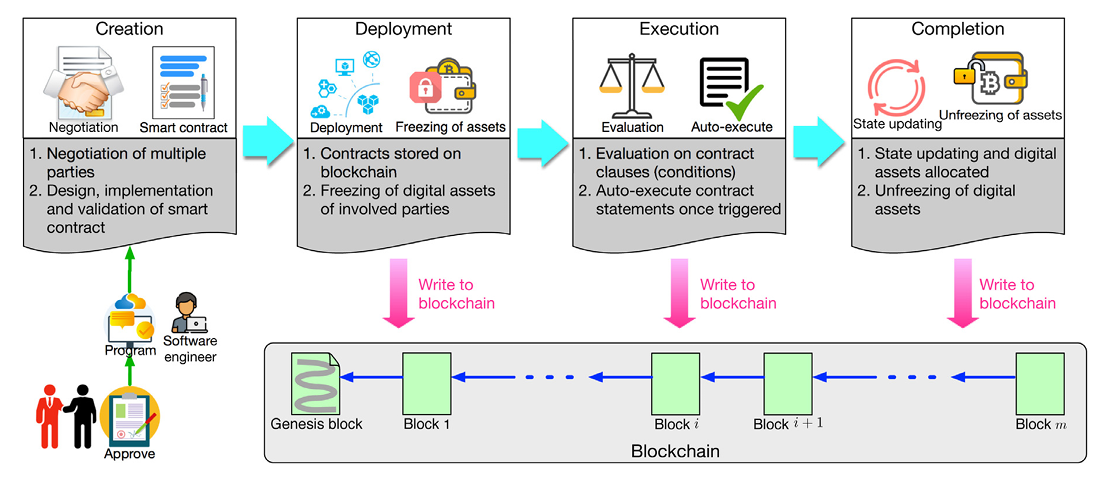
\includegraphics[width=0.7\textwidth]{resources/chapter-2/sc-lifecycle.png}
	\caption{\textit{Life cycle} dari Smart Contract \parencite{zheng2020overview}}
	\label{image:sc-lifecycle}
\end{figure}

\textit{Life cycle} dari sebuah Smart Contract terdiri dari empat fase seperti pada ilustrasi di Gambar \ref{image:sc-lifecycle}:

\begin{enumerate}
	\item \textit{Creation}: negosiasi antar pihak untuk menyepakati ketentuan dari kontrak dalam \textit{natural language}, dan translasi menjadi Smart Contracts.
	\item \textit{Deployment}: kontrak yang sudah divalidasi dapat disimpan ke dalam Blockchain, menjadikannya tidak bisa dimodifikasi.
	\item \textit{Execution}: Setelah \textit{deployment}, klausa kontraktual akan dimonitor, dan saat kondisi yang sesuai dengan yang terdefinisi dalam Smart Contract, maka prosedur kontrak akan dieksekusi secara otomatis.
	\item \textit{Completion}: Setelah eksekusi, \textit{state} baru dari semua pihak akan diperbarui sesuai dengan hasil dari transaksi yang terjadi dan disimpan ke dalam Blockchain. 
\end{enumerate}

\subsection{Smart Contract Sanctuary}
\label{subsec:sc-sanctuary}

Smart Contract Sanctuary adalah sebuah repositori GitHub yang dikembangkan oleh tintinweb dengan tujuan untuk menyediakan kumpulan Smart Contracts yang aman, telah diuji, dan diverifikasi secara menyeluruh untuk digunakan atau dijadikan referensi sehingga dapat mengurangi resiko kerentanan dan bug pada tahap pengembangan Smart Contract \parencite{smart_contract_sanctuary}. 

% \subsection{Off-Chain Smart Contracts}
% \label{subsec:off-chain-smart-contracts}

% \textit{Off-chain Smart Contract} adalah Smart Contracts yang dieksekusi diluar Blockchain, \textit{signed} hanya oleh \textit{interested participants}, dan digunakan untuk mengenkapsulasi fungsi yang melibatkan komputasi \textit{high-cost} atau \textit{private information} terkait \textit{participants}. Terdapat banyak cara untuk tetap menjaga properti dan keuntungan penggunaan dari Blockchain, contohnya, hasil dari eksekusi sebuah \textit{off-chain Smart Contract} dapat dilakukan \textit{logging} pada Blockchain, sehingga jika terjadi \textit{dispute} dalam eksekusi \textit{off-chain Smart Contract}, sebuah \textit{on-chain Smart Contract} dapat digunakan untuk \textit{fork off-chain Smart Contract} dan mengeksekusinya di dalam Blockchain untuk menyelesaikan \textit{dispute} \parencite{zou2019smart}.

\subsection{Semantic Smart Contracts}
\label{subsec:semantic-smart-contracts}
Semantic Smart Contracts adalah sebuah cara untuk merepresentasikan \textit{semantics} dari Smart Contract menggunakan konsep \textit{EthOn contract extension} dan sebuah \textit{vocabulary} yang terkait dengan bisnis. Semantic Smart Contracts mengizinkan untuk membandingkan \textit{request} dengan beberapa \textit{request description} dengan mengonsiderasi semantik dari anotasi yang mereferensikan sebuah \textit{shared domain ontology} \parencite{baqa2019semantic}.

\section{Ontology}
\label{sec:ontology}

Pada tahun 1993, \cite{gruber1993translation} pertama mendefinisikan sebuah ontology sebagai "\textit{explicit specification of a conceptualization}". Pada tahun 1997, \cite{borst1997construction} mendefinisikan ontology sebagai "\textit{formal specification of a shared conceptualization}". Definisi ini menambahkan kebutuhan sebuah ontology sebagai sebuah representasi konseptual yang \textit{shared} diantara beberapa pihak. Sehingga, konseptualisasi tersebut harus diekspresikan dengan sebuah format yang \textit{machine readable}. Sehingga pada tahun 1998, \cite{studer1998knowledge} menggabungkan kedua definisi tersebut sebagai "\textit{an ontology is a formal, explicit specification of a shared conceptualization}."

Dalam tulisannya, \cite{Guarino2009} merangkum ketiga definisi tersebut menjadi: Ontology adalah sebuah \textit{framework} terstruktur untuk merepresentasikan pengetahuan di sebuah \textit{domain} tertentu, seperti mendefinisikan entitas, konsep, dan relasi di dalam \textit{domain} tersebut. Ontology dapat membantu membuat sebuah model yang dapat dimengerti dan dapat dibagikan untuk digunakan dalam berbagai sistem dan aplikasi. Di dalam \textit{domain} sistem informasi, ontology digunakan sebagai sebuah cara formal untuk mengorganisasikan dan merepresentasikan data untuk dibagikan, dilakukan pencarian, dan dilakukan penalaran \parencite{Guarino2009}. 

Beberapa komponen kunci dari sebuah ontology adalah:

\begin{enumerate}
  \item \textit{Classes (Concepts)}: Tipe atau kategori fundamental di dalam sebuah \textit{domain} yang merepresentasikan konsep umum.
  \item \textit{Instances (Individuals)}: Contoh spesifik dari sebuah \textit{class}.
  \item \textit{Properties (Attributes)}: Mendeskripsikan karakteristik dari \textit{classes} atau \textit{instances}.
  \item \textit{Relationships}: Hubungan antar entitas, bisa \textit{hierarchical} atau \textit{associative}.
  \item \textit{Axioms}: Aturan atau \textit{constraint} yang mendefinisikan \textit{valid relationships} dan \textit{properties} di dalam ontology, sehingga dapat dilakukan inferensi logis.
\end{enumerate}

\subsection{The Semantic Web}
\label{subsec:the-semantic-web}

The Semantic Web adalah sebuah ekstensi dari \textit{web} dengan tambahan data dengan arti yang terdefinisi dengan baik, yang diturunkan menggunakan \textit{semantic theory} untuk menginterpretasikan simbol-simbol. \textit{Semantic theory} menyediakan catatan dari arti untuk sebuah istilah atau informasi, sehingga dapat membuat sebuah hubungan logis antar istilah \parencite{shadbolt2006semantic}.

\subsubsection{Universal Resource Identifiers}
\label{subsubsec:universal-resource-identifiers}

Universal Resource Identifiers (URIs) adalah sebuah cara untuk mengidentifikasi sebuah \textit{resource} menggunakan sebuah konvensi penamaan global yang disepakati, sehingga dapat diinterpretasikan secara standar oleh seluruh mesin yang berada di \textit{web}. Saat sebuah \textit{resource} diasosiasikan dengan sebuah URI, maka itu berarti semua orang dapat melakukan \textit{link}, \textit{refer}, dan mengambil \textit{representasi} dari \textit{resource} tersebut menggunakan URI. Skema yang direkomendasikan pada tahun 2004 adalah Resource Definition Framework Schema yang menggunakan spesifikasi dasar dari RDF dengan ekstensi untuk mendukung ekspresi dari \textit{structured vocabularies} \parencite{shadbolt2006semantic}.

\subsubsection{Web Ontology Langugage}
\label{subsubsec:web-ontology-language}

Web Ontology Language (OWL) adalah keluarga bahasa yang dikembangkan oleh World Wide Web Consortium (W3C), digunakan untuk mengembangkan dan berbagi ontologi di dalam \textit{web}. OWL bertujuan untuk memberikan representasi yang efisien untuk ontologi, pengecekan \textit{logical consistency} dan klasifikasi \textit{concept}, menggunakan RDF untuk \textit{linking} sehingga ontologi dapat didistribusikan antar sistem \parencite{shadbolt2006semantic}.

\subsection{Ontology in Blockchain}
\label{subsec:ontology-in-blockchain}

Konsep ontology di dalam blockchain adalah sebuah pendekatan yang berupaya untuk memetakan fitur dan konsep dari blockchain secara formal dan \textit{shared} untuk mendukung \textit{interoperability} \parencite{9770809} dan mewujudkan visi \textit{semantic} blockchain \parencite{hector2020blondie}.

\subsubsection{EthOn}
\label{subsubsec:ethon}

\begin{figure}[ht]
	\centering
	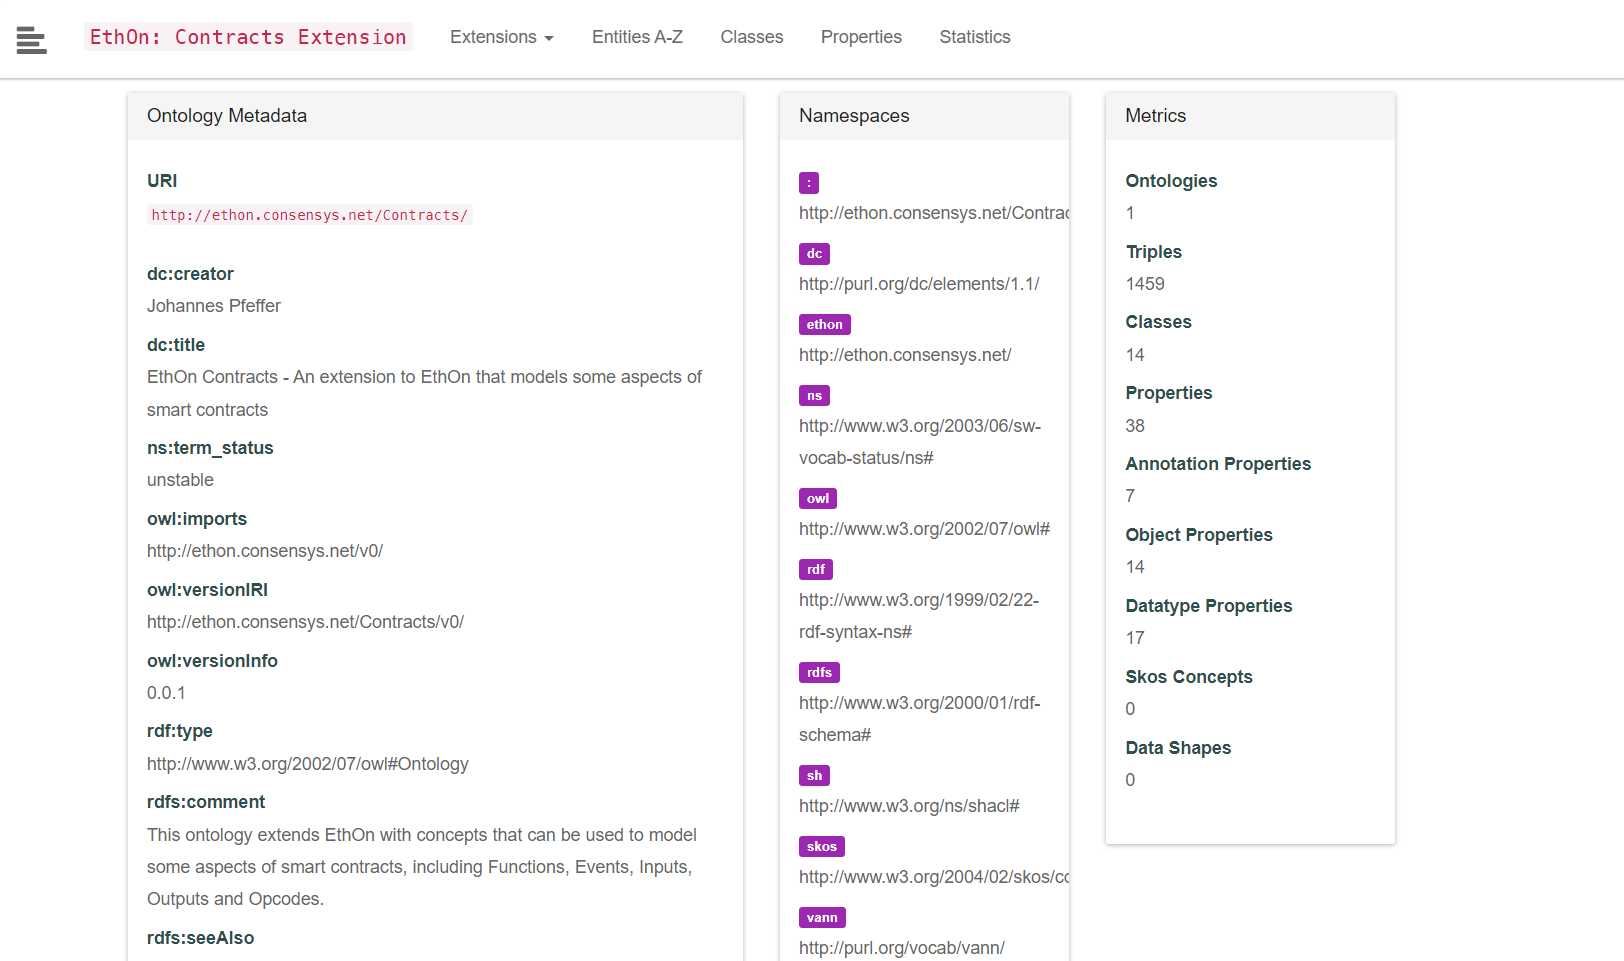
\includegraphics[width=0.7\textwidth]{resources/chapter-2/ethon.png}
	\caption{Visualisasi EthOn \parencite{ethon2024}}
	\label{image:ethon}
\end{figure}

EthOn adalah sebuah ontology yang dirancang secara spesifik untuk ekosistem Ethereum untuk merepresentasikan struktur, komponen, dan relasi di dalam Blockchain Ethereum. Visualisasi EthOn dapat dilihat pada gambar \ref{image:ethon}. EthOn menyediakan \textit{semantic framework} untuk standarisasi dan interpretasi data kompleks yang terasosiasi dengan transaksi, Smart Contracts, blok, akun, dan entitas lainnya. Ontology ini memberikan cara untuk menginterpretasikan data dengan cara yang lebih terstruktur dan berarti, mendukung \textit{interoperability}, dan integrasi data \parencite{pfeffer2016ethon}.

\subsubsection{BLONDiE}
\label{subsubsec:blondie}

\begin{figure}[ht]
	\centering
	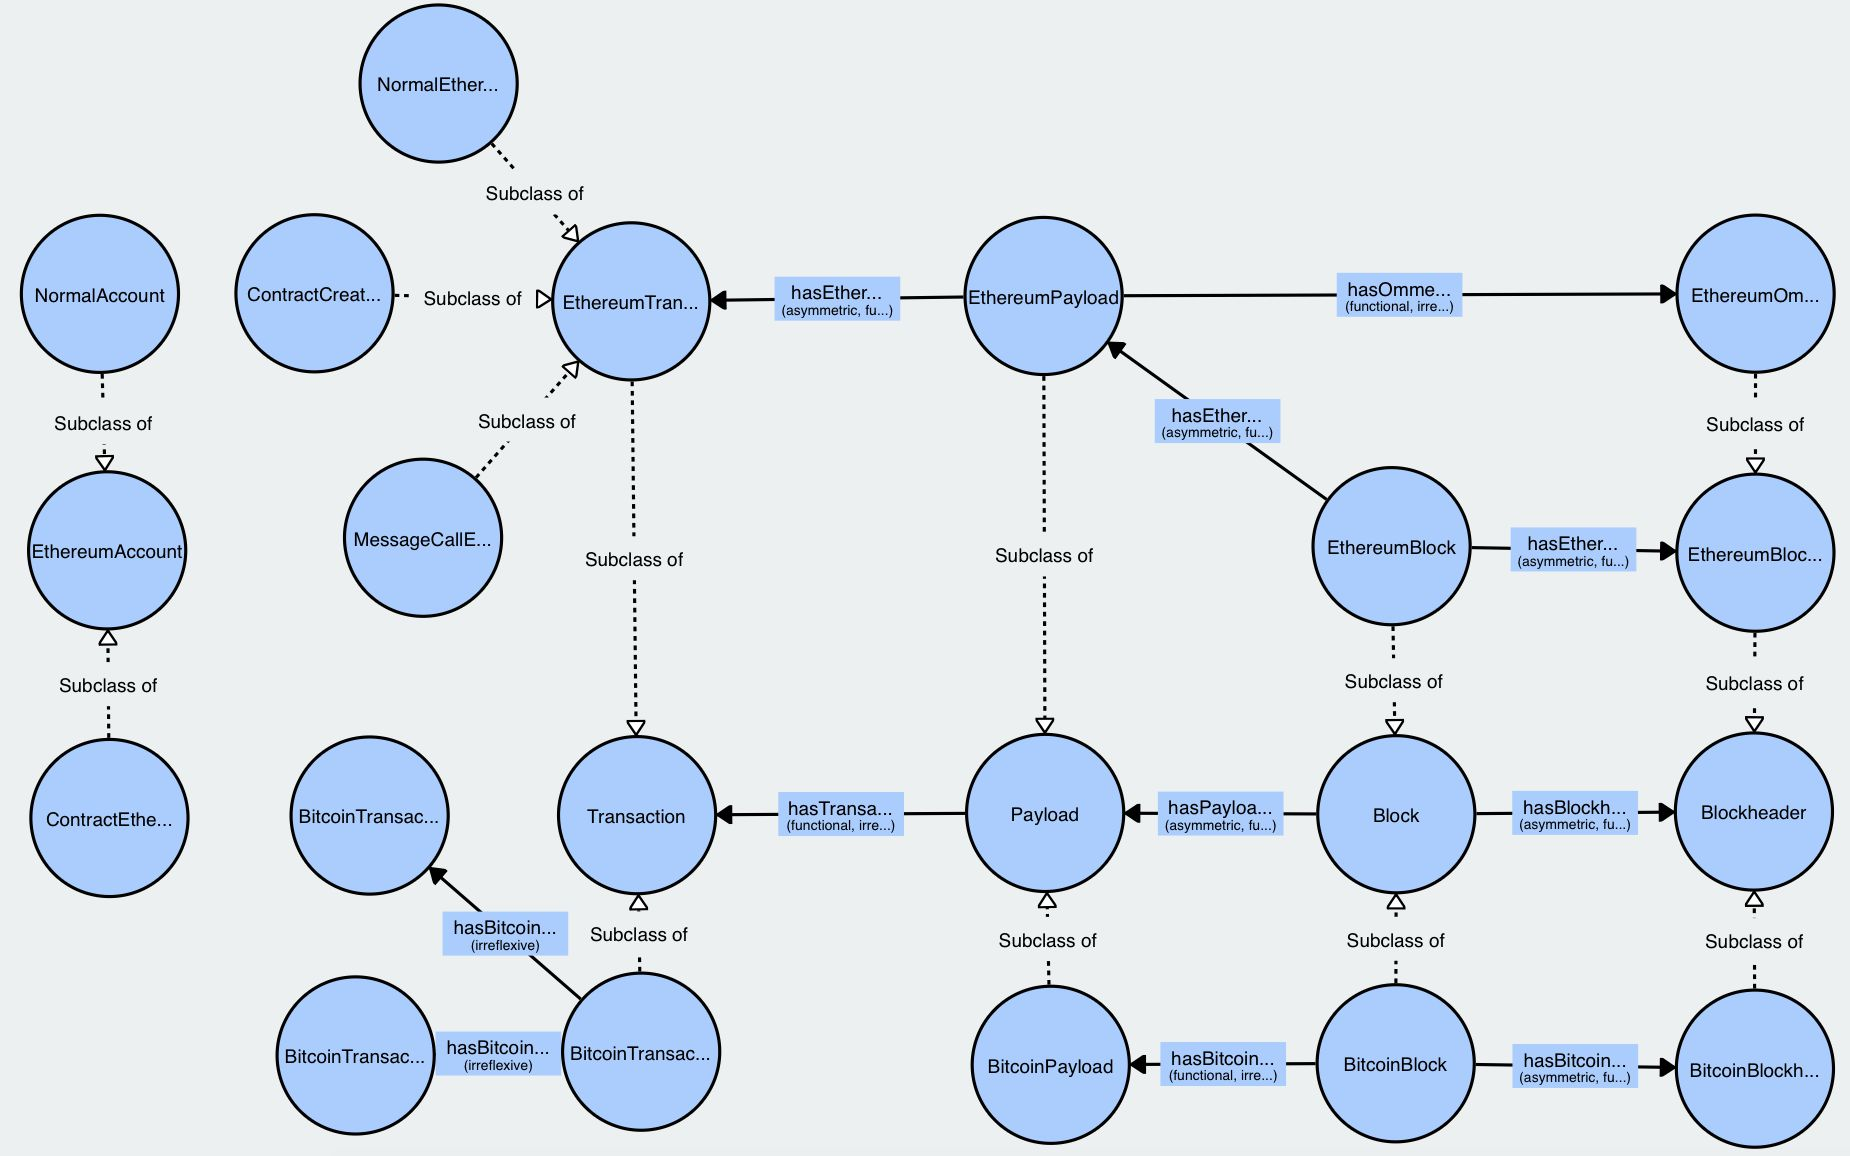
\includegraphics[width=1\textwidth]{resources/chapter-2/blondie-visualization.jpg}
	\caption{Visualisasi Ontology BLONDiE \parencite{third2017linked}}
	\label{image:blondie-visualization}
\end{figure}

BLONDiE adalah singkatan dari blockchain Ontology with Dynamic Extensibility, yang merupakan sebuah \textit{vocabulary} untuk merepresentasikan konsep di dalam blockchain dengan potensi untuk ekstensi. Ontology ini terdiri atas 23 \textit{class}, 11 \textit{object properties}, dan 64 \textit{data properties} \parencite{hector2020blondie}. Gambar \ref{image:blondie-visualization} memvisualisasikan ontology BLONDiE.

\subsection{Minimal Service Model}
\label{subsec:minimal-service-model}

Minimal Service Model adalah sebuah RDF(S) Integration Ontology sederhana berdasarkan prinsip \textit{minimal ontological commitment}, yaitu prinsip dalam perancangan ontologi yang berarti membuat klaim atau asumsi sesedikit mungkin tentang domain yang dimodelkan. Visualisasi dari ontologi MSM dapat dilihat pada gambar \ref{image:msm-visualization}. MSM hanya mendefinisikan struktur dasar seperti Services, Operations, dan Message Content. MSM dikembangkan bukan untuk menambah keragaman model \textit{service} yang sudah ada, melainkan berfungsi sebagai model untuk integrasi yang menjembatani berbagai formalisme yang telah ada. Model ini mampu menangkap semantik inti dari Web Service dan Web API dalam satu model yang sama, sehingga mendukung proses publikasi dan penemuan \textit{service} secara homogen. Salah satu fitur kunci dari MSM adalah kemampuan integrasinya, yang menggunakan properti msm untuk memungkinkan \textit{binding} ke berbagai format deskripsi untuk sebuah \textit{service} seperti WSDL, SWAGGER, WSMO, dan OWL-S, dan juga integrasi \textit{vocabulary} dari ontologi lainnya \parencite{iserve2015datamodel}.

Ekstensi Minimal Service Model antara lain:
\begin{enumerate}
	\item MSM-WSDL \break Memberikan kemampuan \textit{grounding} ke elemen-elemen WSDL.
	\item MSM-SWAGGER \break Memberikan kemampuan \textit{grounding} untuk deskripsi SWAGGER.
	\item MSM-NFP \break Melacak metrik penggunaan \textit{service} yang mencakup informasi terkait properti non-fungsional.
\end{enumerate}

\begin{figure}[ht]
	\centering
	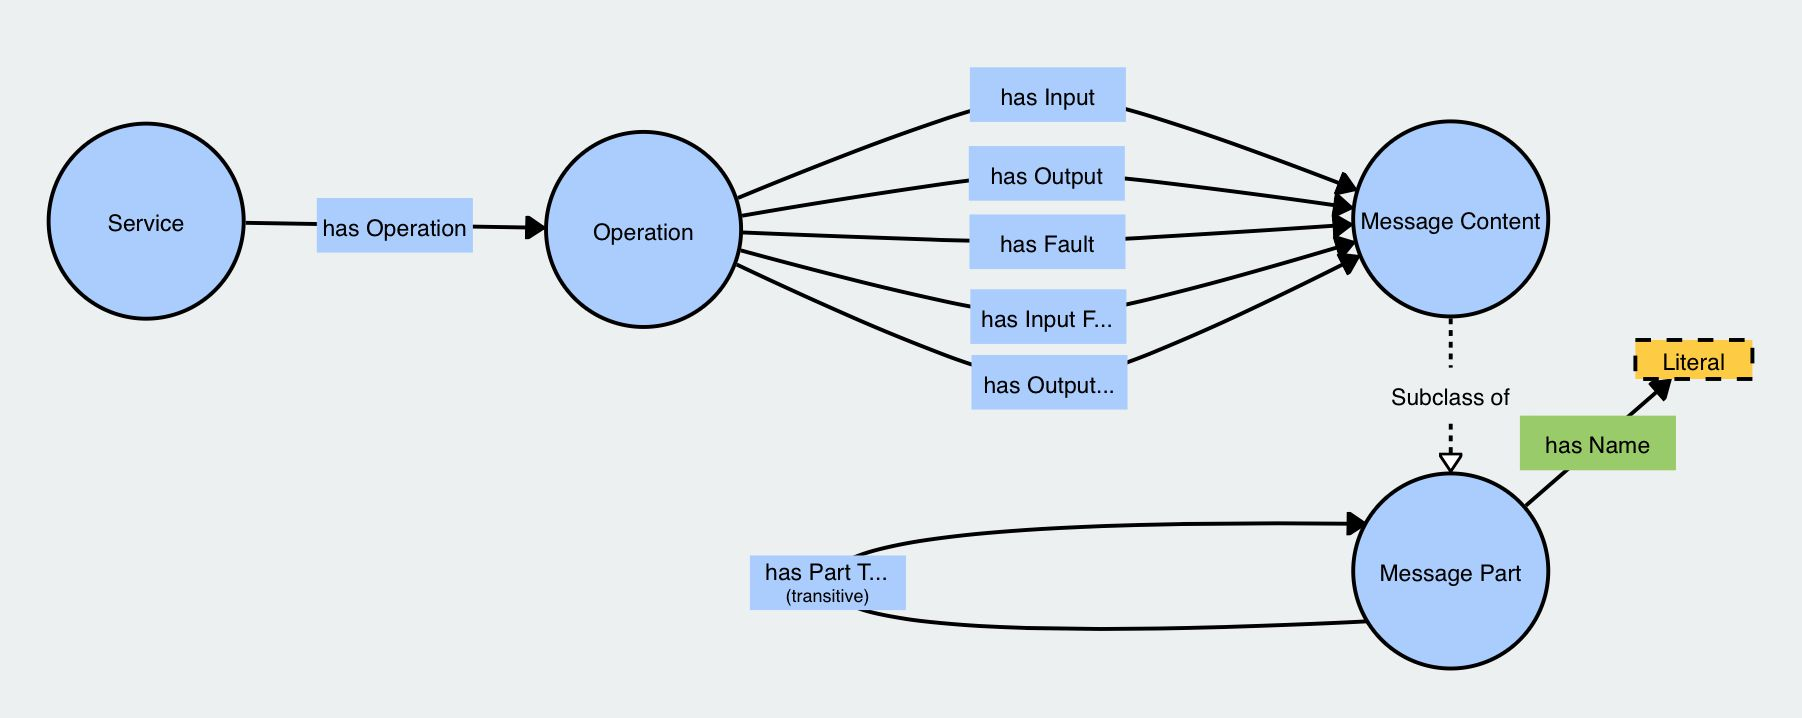
\includegraphics[width=1\textwidth]{resources/chapter-2/msm-visualization.jpg}
	\caption{Visualisasi Ontology Minimal Service Model \parencite{third2017linked}}
	\label{image:msm-visualization}
\end{figure}
% \section{RAG}
\label{sec:rag}

Retrieval Augmented Generation (RAG) adalah sebuah teknik dalam \textit{Artificial Intelligence} yang menggunakan \textit{Natural Language} untuk memperkaya \textit{Large Language Models} dengan pengetahuan eksternal. RAG muncul sebagai solusi dari kekurangan LLM yang selalu menjawab berdasarkan pengetahuan yang kurang relevan atau tidak lengkap. Pendekatan ini memungkinkan model untuk mengambil informasi yang relevan dari dokumen atau basis data tertentu saat berjalan, memperkuat pengetahuan internalnya dan meningkatkan akurasi serta relevansi responsnya \parencite{merritt2025rag}.

Istilah "RAG" pertama kali diperkenalkan oleh \cite{lewis2020retrieval} dari Facebook AI Research, University College London, dan New York University. Dalam makalah tersebut, Lewis dan timnya mengembangkan sebuah model RAG yang mengintegrasikan memori parametrik dan non-parametrik dalam proses generasi bahasa. Memori parametrik berupa model seq2seq (\textit{sequence-to-sequence}) yang telah dilatih sebelumnya, seperti BART, sedangkan memori non-parametrik adalah indeks vektor padat dari Wikipedia yang diakses melalui sistem pengambilan informasi \textit{neural}, seperti \textit{Dense Passage Retriever} (DPR).

\begin{figure}[ht]
  \centering
  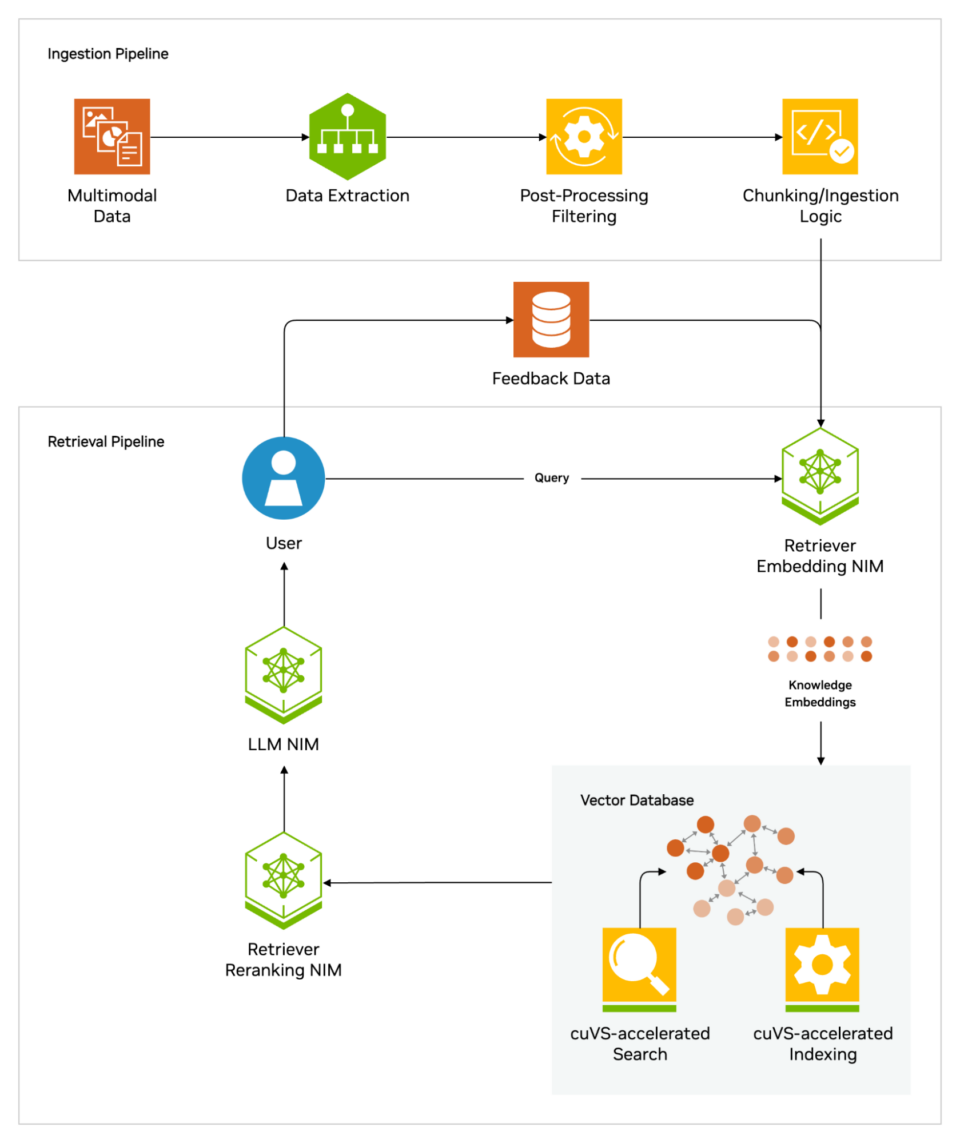
\includegraphics[width=0.7\textwidth]{resources/chapter-2/rag-overview.png}
  \caption{Gambaran umum cara kerja RAG \parencite{merritt2025rag}}
  \label{image:rag-overview}
\end{figure}

\begin{figure}[ht]
  \centering
  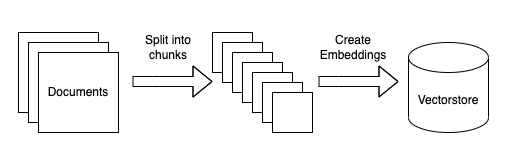
\includegraphics[width=0.7\textwidth]{resources/chapter-2/rag-ingestion.png}
  \caption{Diagram proses ingestion pada RAG \parencite{langchain_chatgpt_data}}
  \label{image:rag-ingestion}
  \end{figure}

\begin{figure}[ht]
  \centering
  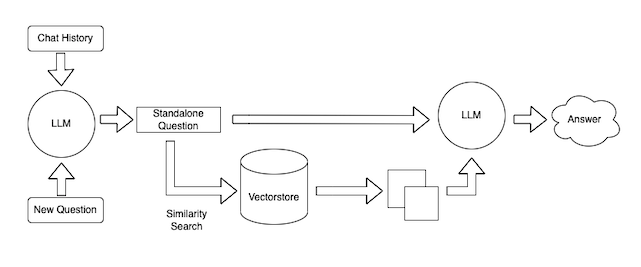
\includegraphics[width=0.7\textwidth]{resources/chapter-2/rag-query.png}
  \caption{Diagram proses query pada RAG \parencite{langchain_chatgpt_data}}
  \label{image:rag-query}
\end{figure}

Cara kerja dari RAG meliputi dua langkah utama, yaitu proses Data Ingestion dan Data Querying, yang dapat didekomposisi menjadi beberapa subproses. Data Ingestion melibatkan pengambilan data dari berbagai sumber, seperti dokumen atau basis data, dan mengubahnya menjadi format standar yang dapat diproses oleh model. Data Querying, di sisi lain, melibatkan pencarian data yang paling relevan dari sumber eksternal berdasarkan query yang diberikan. Proses ini memungkinkan model untuk mengakses informasi tambahan yang diperlukan untuk menghasilkan respons yang lebih akurat dan relevan. Berikut adalah penjelasan dari setiap subproses dalam RAG:

\begin{enumerate}
  \item \textbf{Data Ingestion} \\
  Proses ini melibatkan pengolahan data menjadi format yang dapat digunakan oleh model bahasa. Proses ingesti dapat dibagi menjadi beberapa sub-langkah sebagai berikut:
  \begin{enumerate}
    \item \textbf{Pemuatan Sumber Data ke Teks} \\
    Tahap ini melibatkan pemuatan data dari berbagai sumber (seperti PDF, dokumen, teks, dan lainnya) ke dalam format teks standar. Dalam implementasi LangChain, data dikonversi menjadi objek Document yang berisi teks dan metadata terkait dokumen tersebut.
    \item \textbf{\textit{Chunking} Teks} \\
    Teks yang telah dimuat kemudian dipecah menjadi potongan-potongan kecil (\textit{chunks}). Langkah ini penting karena model bahasa umumnya memiliki batas jumlah teks yang dapat diproses. Dengan membuat potongan teks sekecil mungkin, sistem dapat memilih hanya bagian yang paling relevan untuk digunakan.
    \item \textbf{\textit{Embed} Teks} \\
    Setiap potongan teks diubah menjadi \textit{embeddings} menggunakan model \textit{embedding} seperti OpenAI text-embedding-ada-002. \textit{Embeddings} ini memungkinkan sistem untuk menemukan potongan teks yang paling relevan berdasarkan kesamaan semantik, bukan sekadar kecocokan kata kunci.
    \item \textbf{Membuat \textit{Embeddings} ke Vectorstore} \\
    \textit{Embeddings} dan dokumen terkait kemudian disimpan dalam basis data vektor (vectorstore) seperti FAISS, Pinecone, atau Chroma. Vectorstore membantu dalam pencarian potongan teks yang paling mirip secara cepat dan efisien.
  \end{enumerate}
  \item \textbf{Data Querying} \\
  Proses ini melibatkan penggunaan data yang telah diingesti untuk menjawab pertanyaan pengguna. Proses kueri juga dapat dibagi menjadi beberapa sub-langkah:
  \begin{enumerate}
    \item \textbf{Penggabungan Riwayat Chat dan Pertanyaan Baru} \\
    Sistem menggabungkan riwayat percakapan dengan pertanyaan baru menjadi sebuah pertanyaan mandiri (\textit{standalone question}). Langkah ini penting untuk memungkinkan pengguna mengajukan pertanyaan lanjutan tanpa harus mengulang konteks secara eksplisit.
    \item \textbf{Mencari Dokumen Relevan} \\
    Menggunakan \textit{embeddings} dan vectorstore yang dibuat selama proses ingesti, sistem mencari dokumen yang paling relevan dengan pertanyaan mandiri. Langkah ini memastikan bahwa hanya informasi yang relevan yang digunakan untuk menjawab pertanyaan.
    \item \textbf{Menghasilkan Respon} \\
    Pertanyaan mandiri dan dokumen relevan yang ditemukan kemudian dimasukkan ke dalam LLM untuk menghasilkan respons. Proses ini menggunakan prompt khusus yang disebut QA\_PROMPT, yang dapat disesuaikan untuk memberikan gaya percakapan tertentu pada \textit{chatbot}.
  \end{enumerate}
\end{enumerate}

RAG telah menjadi pendekatan yang sangat populer sejak diperkenalkan untuk meningkatkan kemampuan LLM dalam mengakses dan memanfaatkan informasi dari data internal tanpa perlu melakukan \textit{fine-tuning} model. Dengan menggunakan RAG, aplikasi dapat menjawab pertanyaan berdasarkan dokumen perusahaan, basis pengetahuan, atau \textit{dataset} spesifik domain dengan akurasi yang lebih tinggi dan risiko halusinasi yang lebih rendah.

Implementasi RAG dapat dilakukan menggunakan \textit{framework} seperti LangChain yang menyediakan komponen modular untuk membangun \textit{pipeline} RAG. LangChain menyediakan \textit{interface} sederhana untuk berinteraksi dengan \textit{chatbot} melalui terminal (CLI) dan juga memungkinkan \textit{deployment} menggunakan Gradio untuk \textit{interface} web. Dengan pendekatan modular ini, setiap komponen dalam \textit{text} RAG dapat disesuaikan atau diganti sesuai dengan kebutuhan spesifik aplikasi.


% \section{Distributed Graph}
\label{sec:dgraph}
\section{Penelitian dan Riset Terkait}
\label{sec:penelitian-riset-terkait}

Berikut merupakan riset dan penelitian yang selaras dan juga menjadi komponen pendukung bagi tugas akhir ini.

% ekstraksi data
\subsection{Extraction, indexing, and analysis of Ethereum Smart Contracts data}
\label{subsec:extraction-indexing-analysis-ethereum-sc}

\begin{figure}[ht]
	\centering
	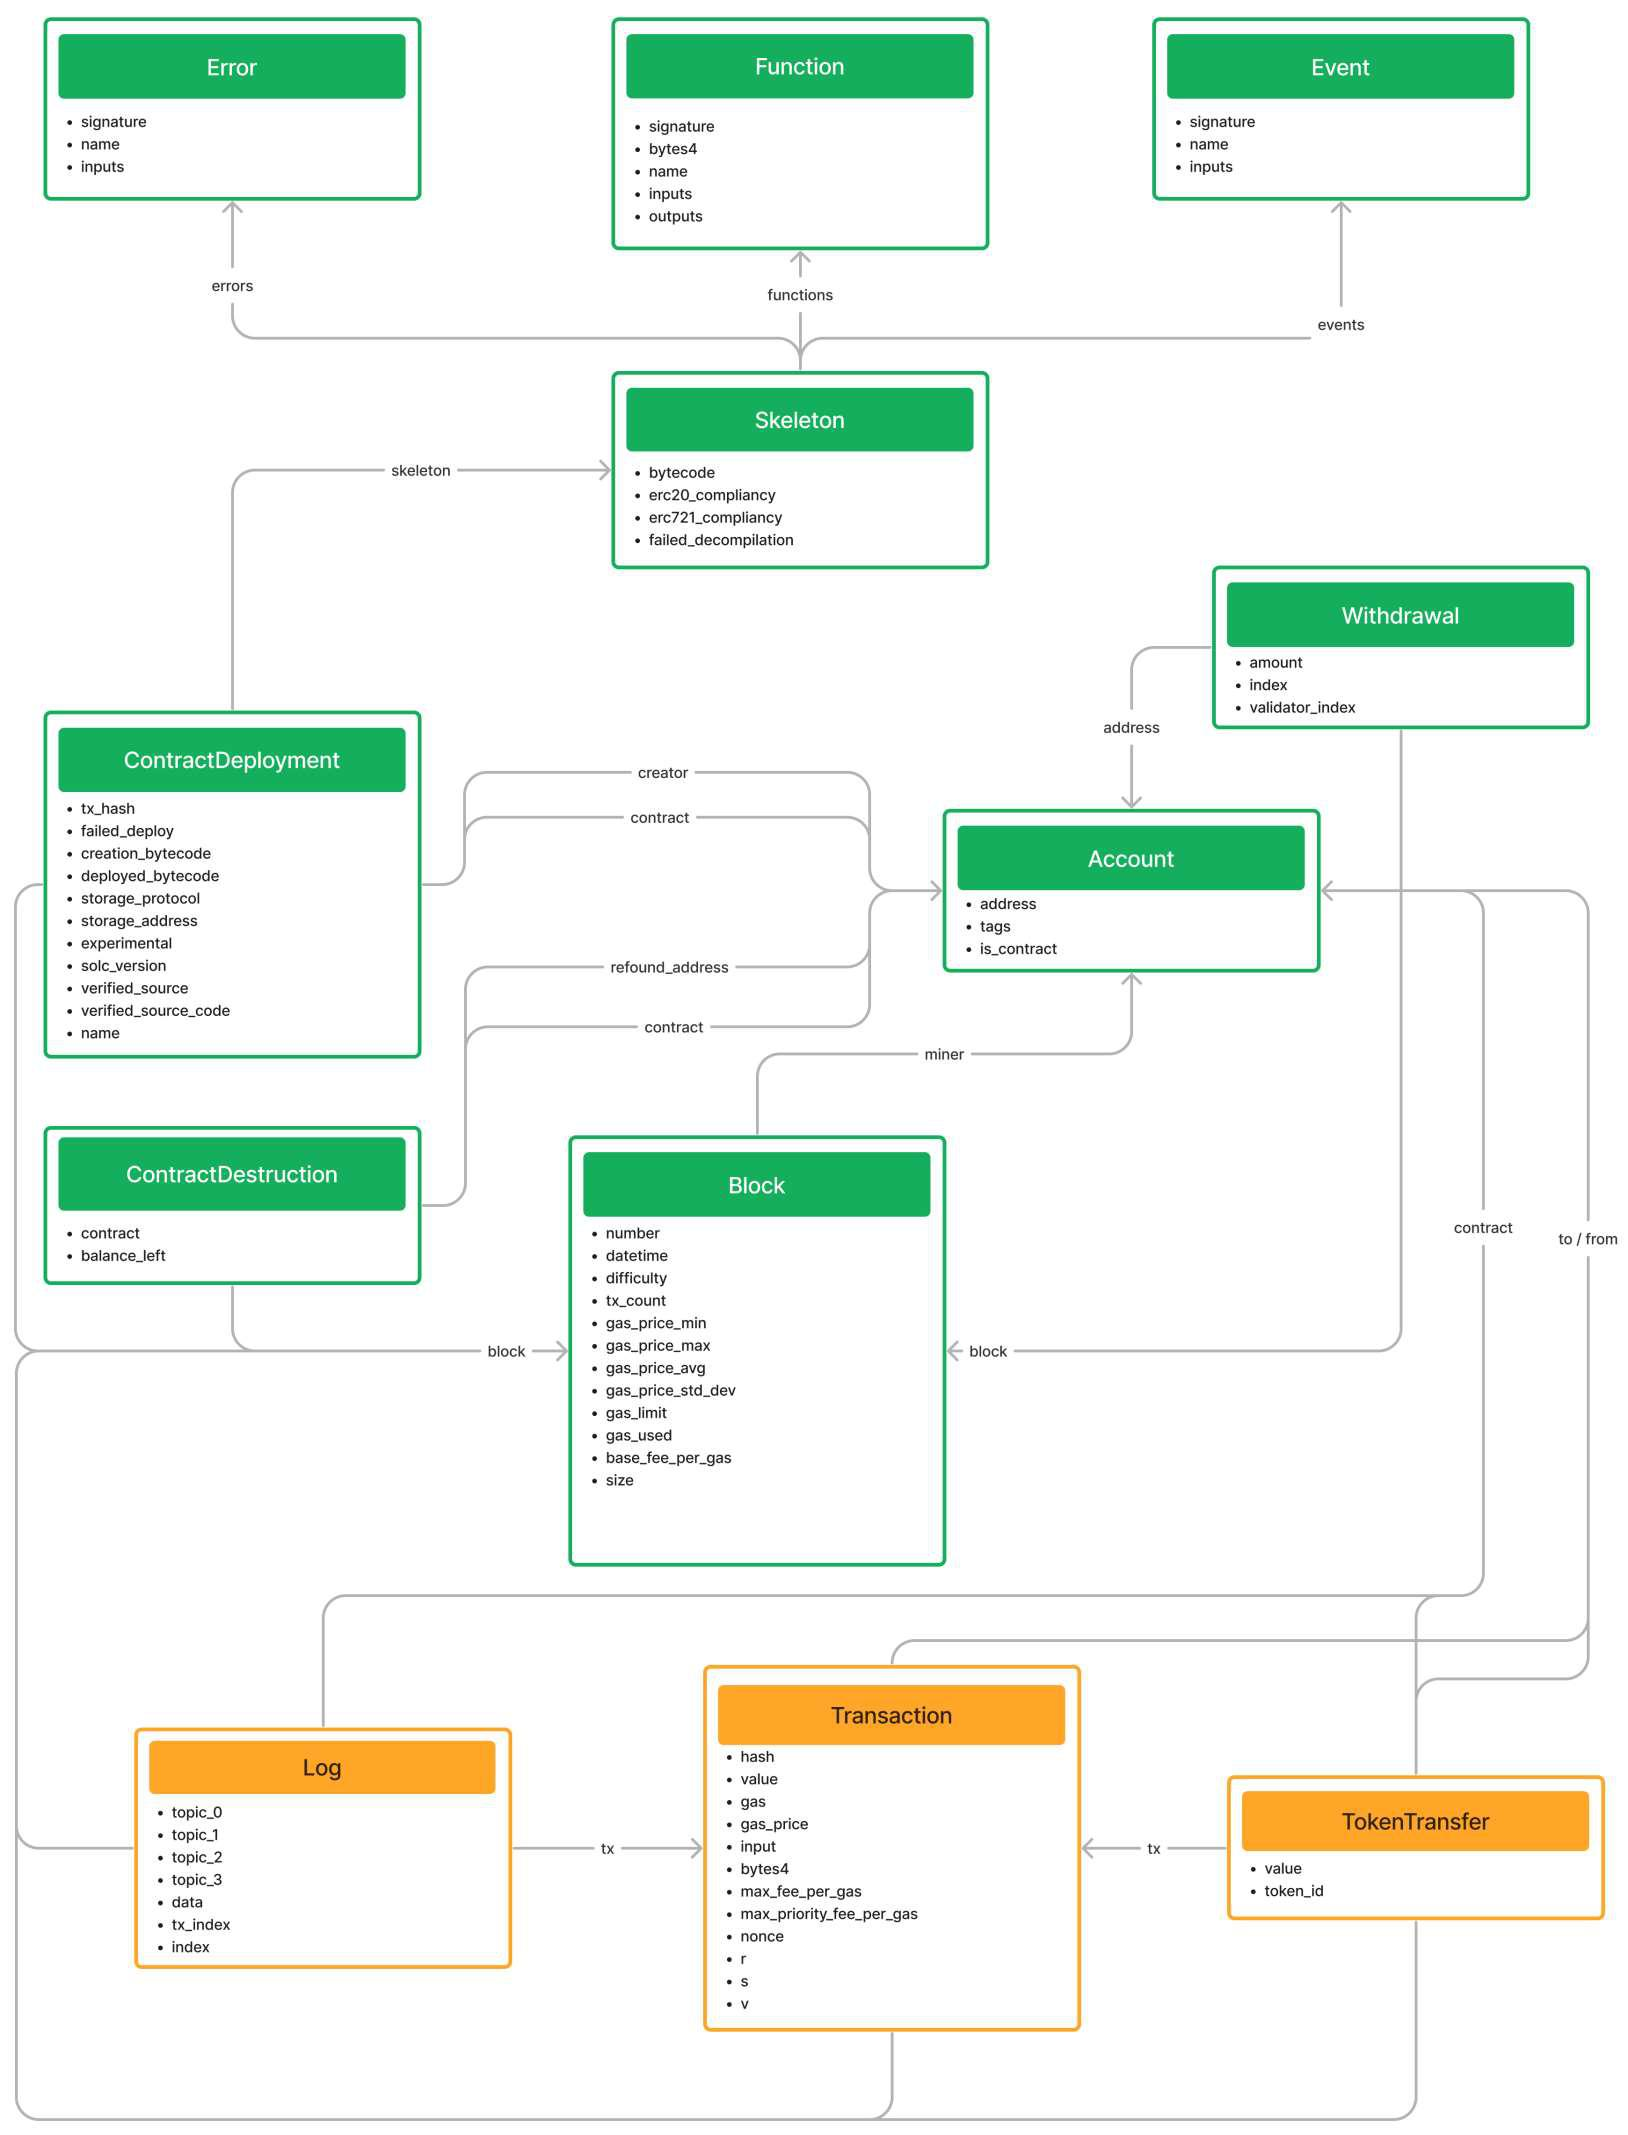
\includegraphics[width=0.7\textwidth]{resources/chapter-2/eth2dgraph-structure.jpg}
	\caption{Data model eth2dgraph \parencite{aimar2023extraction}}
	\label{image:eth2dgraph-structure}
\end{figure}

Penelitian yang dilakukan sebagai \textit{thesis} oleh \cite{aimar2023extraction} berfokus pada bagaimana mengambil data dari Blockchain Ethereum yang bersifat publik, mengekstrasi semantiknya, lalu mentransformasikannya ke sebuah bentuk yang mudah diakses oleh pengguna dengan cara mengindeksnya menggunakan Dgraph, sebuah \textit{open-source distributed graph database}. Hasil dari penelitian ini adalah sebuah perangkat lunak bernama eth2dgraph, yang ditulis dalam bahasa Rust yang melakukan mapping data Ethereum ke format Dgraph, dengan data model yang ditunjukkan pada gambar \ref{image:eth2dgraph-structure}. Perangkat lunak ini mengintegrasikan sebuah \textit{decompiler} untuk mengekstraksi dan mengindeks ABI dari Smart Contracts.

Beberapa hal yang dapat diperhatikan dari perangkat lunak eth2dgraph adalah:

\begin{enumerate}
	\item Ekstraksi ABI \newline Cara eth2dgraph mengekstraksi semantik dari sebuah Smart Contract yang sudah dalam bentuk EVM Bytecode, yaitu dalam ABI (\textit{Application Binary Interface}). Gambar \ref{image:abi-extraction} menggambarkan bagaimana eth2dgraph memanfaatkan heimdall-rs untuk melakukan dekompilasi ABI. Cara ini dapat mengekstraksi lokasi fungsi, informasi terkait tipe \textit{input} dan \textit{output} dan nama fungsi, tetapi tidak memungkinkan untuk mengekstraksi nama parameter karena sudah dihilangkan pada saat kompilasi.
	      \begin{figure}[ht]
		      \centering
		      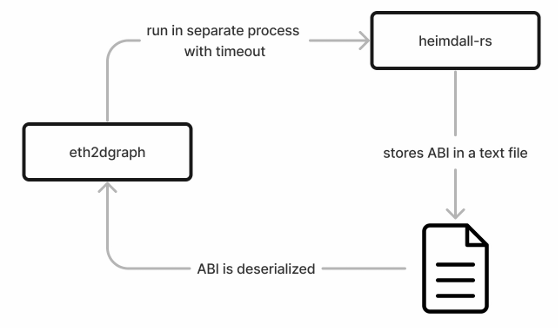
\includegraphics[width=0.7\textwidth]{resources/chapter-2/eth2dgraph-heimdall.png}
		      \caption{Ekstraksi ABI \parencite{aimar2023extraction}}
		      \label{image:abi-extraction}
	      \end{figure}
	\item Ekstraksi struktur dan metadata \newline Cara eth2dgraph mengekstraksi struktur Smart Contract dan metadata adalah menggunakan Regular Expression, dengan bagian \textit{runtime} diproses untuk mengekstraksi struktur, sedangkan bagian metadata dilakukan \textit{decode}.
	\item Ekstraksi menggunakan source code \newline eth2dgraph juga dapat melakukan ekstraksi semantik menggunakan source code yang tersedia dari sebuah Smart Contract, dengan cara melakukan query terhadap teks yang ada di dalam Smart Contract.
\end{enumerate}

\subsection{Ethereum ETL}
\label{subsec:ethereum-etl}

Ethereum ETL (Extract, Transform, Load) adalah sebuah kakas yang dirancang untuk mengekstraksi, mentransformasi, dan memuat data dari blockchain Ethereum. Kakas ini ditujukan bagi pengembang dan analis yang ingin mengakses serta memproses data blockchain, memungkinkan integrasi ke dalam basis data atau alat analisis lainnya. 

Dikembangkan oleh tim Blockchain ETL, sistem ini menyediakan serangkaian alat untuk:

\begin{enumerate}
  \item Ekspor Data Ethereum: Mendukung ekspor blok Ethereum, transaksi, transfer token ERC20/ERC721, transaksi internal, log, dan data kontrak ke dalam format yang mudah diakses seperti file CSV atau basis data relasional.
  \item Streaming Data: Ethereum ETL memungkinkan streaming data blockchain secara \textit{real-time}, memberikan akses langsung ke transaksi, blok, dan transfer token Ethereum.
  \item Integrasi BigQuery: Pustaka ini menyediakan cara mudah untuk mengunggah dan menjalankan kueri terhadap data Blockchain Ethereum melalui Google BigQuery, memfasilitasi analisis data dalam skala besar.
\end{enumerate}

Arsitektur sistem yang dirancang untuk fleksibilitas memungkinkan pengguna untuk mengatur pekerjaan ETL untuk kumpulan data Ethereum, dan menyediakan cara yang efisien untuk menganalisis atau memvisualisasikan data Blockchain. Sebagai \textit{open-source software}, Ethereum ETL membantu pengguna berinteraksi dengan data Ethereum tanpa memerlukan pengaturan infrastruktur Blockchain yang kompleks. \parencite{ethereum_etl}
\subsection{Xblock-ETH}
\label{subsec:xblock-eth}

\cite{zheng2020xblock} mempublikasikan sebuah \textit{dataset} data mentah dari Blockchain Ethereum, dan mengusulkan sebuah \textit{framework} yang digunakan untuk mendapatkan data tersebut, yang disebut Xblock-ETH. Data dilakukan \textit{update} secara periodik dalam \textit{chunk} berjumlah 500,000 blok. \textit{Dataset} ini terbagi menjadi beberapa \textit{dataset} yang lebih kecil yang meliputi: \textit{block}, \textit{block transaction}, \textit{internal transaction}, \textit{contract info}, \textit{ERC20 transaction}, \textit{ERC721 transaction}, dan \textit{token info}.

Xblock-ETH menyediakan alternatif untuk mendapatkan data tanpa menjalankan sebuah \textit{node} Ethereum, yang memerlukan waktu dan sumber daya yang besar. Tetapi kekurangan dari Xblock-ETH adalah terdapat kekurangan informasi yang penting seperti \textit{logs} dan \textit{receipts}. Secara penggunaan, Xblock-ETH dinilai kurang mudah untuk digunakan karena memerlukan \textit{parsing} data CSV yang banyak, yang tidak mudah dilakukan query atau \textit{index}.



% pemodelan, penyimpanan, indexing
\subsection{Linked Data Indexing of Distributed Ledgers}
\label{subsec:linked-data-indexing-distributed-ledgers}

Penelitian yang dilakukan oleh \cite{third2017linked} membahas tantangan dalam pencarian informasi pada \textit{distributed ledger}, yang sulit dilakukan karena informasi mengenai suatu entitas dapat tersebar di seluruh \textit{ledger} tanpa adanya indeks. Penelitian ini mengusulkan penggunaan indeks berbasis semantik untuk Ethereum Blockchain dengan pendekatan \textit{Linked Data}, yang memungkinkan pencarian menggunakan istilah khusus sesuai \textit{domain}. Pendekatan ini diharapkan dapat meningkatkan kekuatan, kegunaan, dan cakupan dari sistem \textit{ledger} tersebut.

Dalam penelitian ini, mereka mengimplementasikan indeks semantik pada Ethereum Blockchain untuk mengekspos data di dalam \textit{distributed ledger} sebagai \textit{Linked Data}. Indeks ini mengindeks data pada level blok dan transaksi menggunakan ontologi BLONDiE, serta memetakan Smart Contract ke dalam ontologi \textit{Minimal Service Model} (MSM) sebagai langkah awal untuk menghubungkan Smart Contract dengan \textit{Semantic Web Services}.

Implementasi indeks semantik ini menggunakan ontologi BLONDiE sebagai kerangka untuk mengelompokkan dan mendeskripsikan elemen-elemen utama dari Blockchain. Ontologi \textit{Minimal Service Model}, yang biasanya digunakan untuk \textit{web services}, diterapkan untuk menggambarkan fungsionalitas dari Smart Contract pada Blockchain, sehingga memungkinkan integrasi yang lebih efisien.

\begin{figure}[ht]
  \centering
  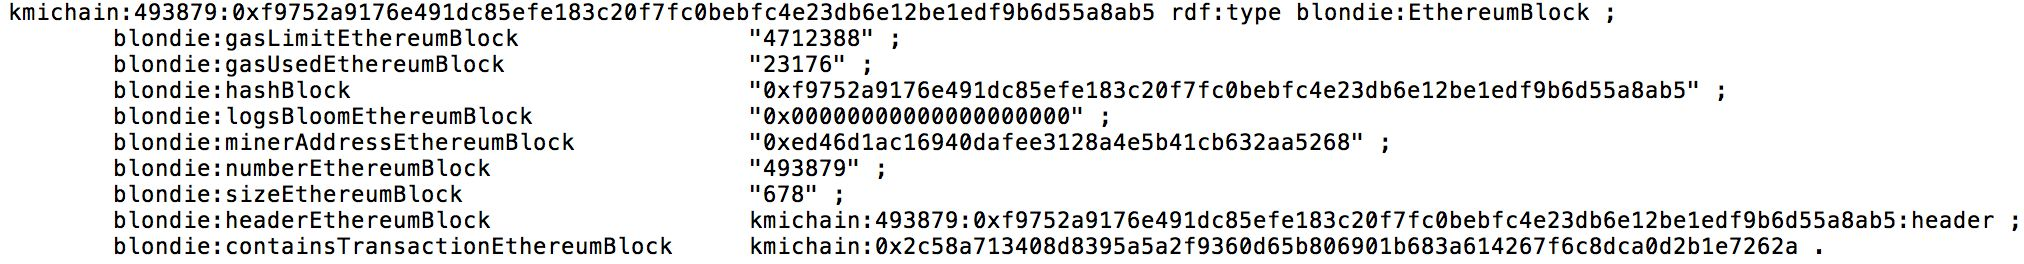
\includegraphics[width=1\textwidth]{resources/chapter-2/rdf-block.jpg}
  \caption{RDF dari deskripsi blok \parencite{third2017linked}}
  \label{image:rdf-block}
\end{figure}

\begin{figure}[ht]
  \centering
  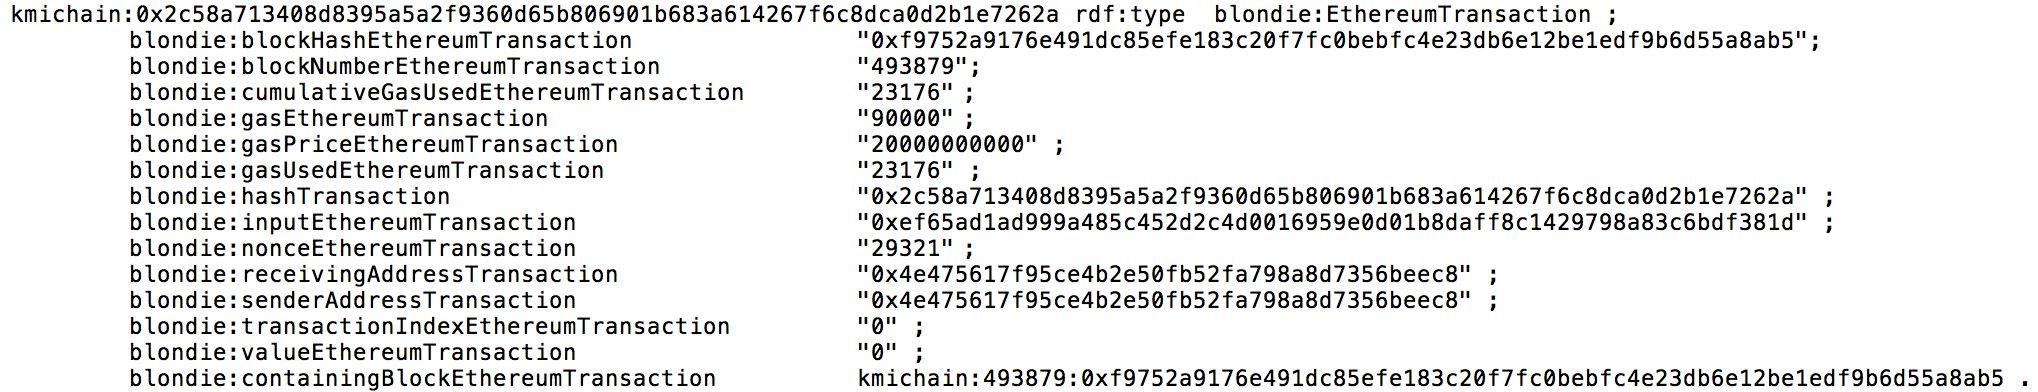
\includegraphics[width=1\textwidth]{resources/chapter-2/rdf-transaction.jpg}
  \caption{RDF dari deskripsi transaksi \parencite{third2017linked}}
  \label{image:rdf-transaction}
\end{figure}

Proyek ini diimplementasikan pada jaringan Ethereum Blockchain privat, di mana komponen \textit{listener} dikembangkan untuk mendeteksi blok baru dan mengindeksnya berdasarkan ontologi BLONDiE. RDF \textit{triples} kemudian dihasilkan dari data ini, yang memungkinkan penguraian data Blockchain secara semantik untuk mendukung pencarian data yang lebih terstruktur. Gambar \ref{image:rdf-block} dan gambar \ref{image:rdf-transaction} adalah contoh dari RDF \textit{triples} yang dihasilkan dari deskripsi blok dan transaksi masing-masing.

Hasil dari penelitian ini menunjukkan bahwa \textit{semantic indexing} memungkinkan data di dalam Blockchain menjadi lebih mudah diakses dan dapat terintegrasi dengan sumber data eksternal. Hal ini membuka peluang untuk mengembangkan \textit{semantic indexing} pada platform Blockchain lainnya serta berpotensi memperluas interoperabilitas data antara Blockchain dan \textit{Semantic Web}.
\subsection{The Graph Protocol}
\label{subsec:the-graph-protocol}

Produk yang dikembangkan oleh \cite{TheGraphDocs}, The Graph, adalah sebuah protokol indeksasi terdesentralisasi untuk data blockchain yang memungkinkan pengguna untuk mendapatkan data terstruktur dari blockchain lainnya melalui antarmuka GraphQL. Sebelumnya, sulit atau bahkan tidak mungkin bagi pengguna untuk mendapatkan hasil operasi query tingkat lanjut dari data Smart Contracts tertentu seperti agregasi atau relasi. The Graph menyelesaikan permasalahan ini dengan sebuah protokol terdesentralisasi yang melakukan indeksasi data pada Blockchain Ethereum menggunakan subgraphs. Subgraphs merupakan koleksi data independen yang mengindeks subset kecil dari jaringan blockchain. Umumnya, subgraph mengindeks data dari satu atau beberapa Smart Contracts yang merupakan bagian dari protokol umum, seperti Uniswap. Semua subgraph yang tersedia dapat ditemukan di Graph Explorer.

Data diindeks dengan menggunakan subgraph manifest, sebuah file YAML yang berisi deskripsi dari bagian-bagian yang diperlukan oleh subgraph, termasuk pemetaan data Ethereum dan log yang terkait. Semua bagian ini diorganisir dengan baik agar dapat diakses oleh berbagai aplikasi terdesentralisasi (dApp), mengurangi ketergantungan pada layanan data terpusat dan memperkenalkan mekanisme yang lebih terbuka dan terdesentralisasi.

Protokol ini melibatkan beberapa aktor utama:

\begin{itemize}
	\item Pengembang: Mereka yang memiliki pengetahuan teknis untuk mengembangkan kode yang diperlukan untuk membuat dan memelihara indeks, seperti pemetaan dari acara Ethereum ke data yang disimpan, yang ditulis dalam AssemblyScript.
	\item Indexers: Bertanggung jawab untuk mengoperasikan \textit{node} dan melayani kueri dari pengguna. Untuk mengindeks dan melayani kueri, indexers harus mempertaruhkan minimal 100.000 token GRT (setara dengan sekitar 12.000 USD). Mereka diberi hadiah dalam bentuk token GRT berdasarkan jumlah kueri yang dilayani.
	\item Curators: Bertugas untuk menemukan subgraphs terbaik yang harus diindeks.
	\item Delegators: Mengamankan jaringan dengan mengunci nilai ekonomi ke indexers tertentu yang mereka pilih, memberikan mereka kemungkinan untuk melayani lebih banyak kueri.
\end{itemize}

Sistem ini beroperasi dengan mata uang GRT yang digunakan dalam ekonomi token, memberikan insentif ekonomi untuk para aktor yang terlibat agar berperilaku baik dan memastikan kualitas layanan. Dengan demikian, The Graph menjadi protokol pertama yang mencoba mendesentralisasi indeksasi data blockchain, yang sangat penting untuk masa depan Web3 dan dApps yang tidak bergantung pada layanan data terpusat.
% graphchain

% klasifikasi fungsional dan semantik
\subsection{Semantic Smart Contracts for Blockchain-based Services in the Internet of Things}
\label{subsec:semantic-smart-contract-iot}

Penelitian yang dilakukan oleh \cite{baqa2019semantic}, mengusulkan sebuah solusi untuk menemukan dan menggunakan Smart Contract untuk kegunaan spesifik, yang sulit dilakukan karena Smart Contract biasanya sudah dikompilasi dalam bentuk \textit{byte-code}, tanpa metadata yang terasosiasi. Solusi yang diusulkan adalah Semantic Smart Contract yang mengintegrasikan RESTful Semantic Web Technologies dalam Smart Contract, yang di-\textit{deploy} pada Blockchain Ethereum untuk melakukan \textit{indexing}, \textit{browsing}, dan melakukan anotasi terhadap sebuah Smart Contract. Penelitian ini menggunakan penelitian \cite{third2017linked} terkait Linked Data Indexing untuk meningkatkan \textit{discoverability}.

\begin{figure}[ht]
	\centering
	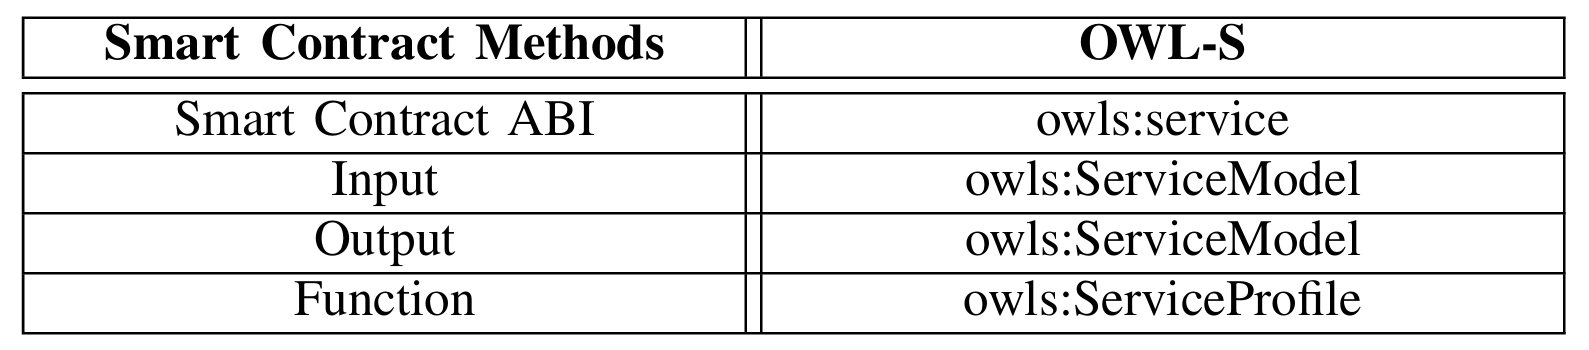
\includegraphics[width=0.7\textwidth]{resources/chapter-2/ssc-ontology-extension.png}
	\caption{Ekstensi OWL-S \parencite{baqa2019semantic}}
	\label{image:ekstensi-owl-s}
\end{figure}

Dalam pengembangan solusi yang diusulkan dalam penelitian ini, dilakukan ekstensi pada OWL-S Service Ontology, seperti pada gambar \ref{image:ekstensi-owl-s} dengan menginkorporasikan beberapa terminologi yang \textit{domain specific} seperti yang ada di dalam EthOn. Sehingga, Semantic Smart Contract dapat digunakan untuk memperkaya query untuk sebuah terminologi yang \textit{domain specific} antar beberapa \textit{distributed ledgers}, yang meningkatkan \textit{discoverability} dari sebuah aplikasi IoT yang terdesentralisasi.
\subsection{Ontological Modeling of Smart Contracts in Solidity}
\label{subsec:solidity-ontology}

Formalisasi menggunakan ontology berbasis domain baru dilakukan pada Blockchain dan Smart Contract, tetapi belum ada yang dilakukan terhadap bahasa pemrograman Smart Contract itu sendiri. Pada penelitiannya, \cite{cano2021toward} mengusulkan sebuah representasi dari bahasa pemrograman Smart Contract yang terkemuka, yaitu Solidity, dengan mendefinisikan semua entitas yang dibutuhkan untuk mencakup seluruh bahasa dan menyelaraskan ke ontology terstandarisasi lainnya seperti EthOn.

Beberapa spesifikasi yang dituliskan di dalam penelitian ini:

\begin{enumerate}
  \item Implementasi Solidity Library
  \item Implementasi Solidity Contract
  \item Interface dan Abstract Contract Solidity
  \item Spesifikasi Attributes dan representasinya di dalam Ontology 
  \item Spesifikasi Types dan representasinya di dalam Ontology
  \item Spesifikasi Constructor dan representasinya di dalam Ontology
  \item Spesifikasi Function dan representasinya di dalam Ontology
  \item Spesifikasi Modifier dan representasinya di dalam Ontology
  \item Spesifikasi Receive dan representasinya di dalam Ontology
  \item Spesifikasi Fallback dan representasinya di dalam Ontology
  \item Spesifikasi Event dan representasinya di dalam Ontology
\end{enumerate}
\subsection{STAN: Towards Describing Bytecodes of Smart Contract}
\label{subsec:stan}

Penelitian yang dilakukan oleh \cite{stan} mengusulkan sebuah sistem bernama STAN untuk melakukan deskripsi terhadap \textit{bytecodes} dari Smart Contracts. STAN merupakan sebuah sistem yang dirancang untuk mengatasi masalah dalam mengekstraksi informasi dari \textit{bytecodes} yang dihasilkan oleh kompilator Solidity. Untuk setiap \textit{interface}, terdapat empat kategori deskripsi yang dapat dihasilkan, yaitu: \textit{functionality description}, \textit{usage description}, \textit{behaviour description}, dan \textit{payment description}. STAN bekerja dengan memanfaatkan \textit{symbolic execution} dan \textit{Natural Language Processing} (NLP) untuk menghasilkan deskripsi yang lebih mudah dipahami oleh pengguna.

\begin{figure}[ht]
	\centering
	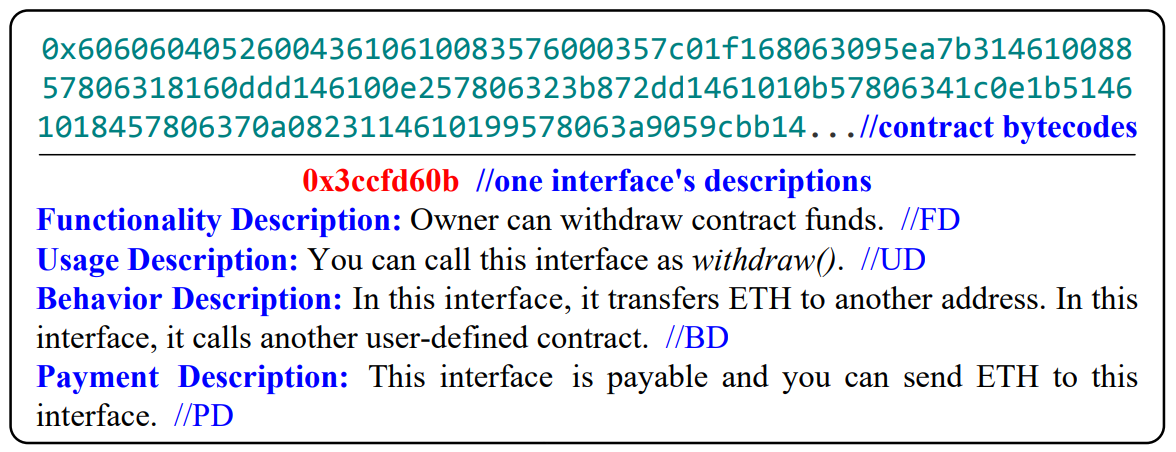
\includegraphics[width=0.7\textwidth]{resources/chapter-2/stan-desc.png}
	\caption{Hasil deskripsi dari STAN untuk Bytecode salah satu \textit{closed-source} Smart Contract \parencite{stan}}
	\label{image:stan-desc}
\end{figure}

\begin{figure}[ht]
	\centering
	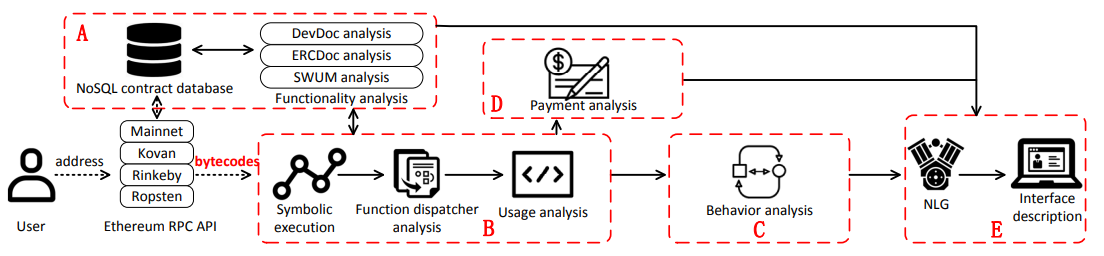
\includegraphics[width=0.7\textwidth]{resources/chapter-2/stan-architecture.png}
	\caption{Arsitektur sistem STAN \parencite{stan}}
	\label{image:stan-architecture}
\end{figure}

Arsitektur dari STAN (Gambar \ref{image:stan-architecture}) terdiri dari beberapa modul utama, yaitu:

\begin{enumerate}
	\item \textbf{Functionality Analysis Module} \\
	      Modul ini melakukan analisis terhadap kontrak melalui teknik \textit{Natural Language Processing} (NLP) untuk menghasilkan frasa yang terkait dengan fungsionalitas dari \textit{interface} kontrak. Fungsionalitas utama dari modul ini adalah untuk mendeskripsikan Bytecode \textit{closed-source contracts}, sementara kontrak \textit{open-source contracts} dan metadata dianalisis untuk membantu analisis Bytecode dengan menemukan \textit{byte signatures} yang identik.

	\item \textbf{Usage Analysis Module} \\
	      Modul ini mengekstrak \textit{byte signatures} fungsi dari \textit{dispatcher} fungsi dan mengembalikan \textit{signature} teks yang sesuai. Dari \textit{signature} teks (misalnya \texttt{transfer(address, uint256)}), pengguna dapat mengetahui nama fungsi dan konfigurasi parameter yang digunakan untuk memanggil \textit{interface}. Modul ini memungkinkan pemahaman yang lebih baik mengenai bagaimana fungsi digunakan dalam kontrak.

	\item \textbf{Behavior Analysis Module} \\
	      Modul ini menganalisis fungsi eksternal/publik untuk menghasilkan informasi perantara terkait perilaku panggilan pesan menggunakan \textit{symbolic execution}. Dengan menganalisis opcode dan operand, modul ini dapat mengenali empat jenis perilaku sensitif dalam panggilan pesan, seperti transfer ETH, penerapan kontrak, dan panggilan kontrak.

	\item \textbf{Payment Analysis Module} \\
	      Modul ini menganalisis fungsi eksternal/publik untuk menghasilkan informasi perantara terkait fitur pembayaran melalui \textit{symbolic execution}. Dengan membangun \textit{Control Flow Graph} (CFG), modul ini dapat mengenali dua pola pembayaran yang menunjukkan apakah \textit{interface} tersebut dapat melakukan pembayaran atau tidak.

	\item \textbf{NLG Module} \\
	      Modul ini menghasilkan deskripsi \textit{interface} yang dapat dibaca dengan memanfaatkan hasil dari empat modul sebelumnya. Proses \textit{Natural Language Generation} (NLG) mengikuti alur standar sistem NLG, yaitu \textit{document planner}, \textit{microplanner}, dan \textit{surface realizer}, untuk menghasilkan deskripsi \textit{interface} yang mudah dipahami oleh pengguna.
\end{enumerate}

STAN dikembangkan pada tahun 2020, dan mencapai hasil yang sangat baik dalam melakukan deskripsi Smart Contract yang bersifat \textit{closed-source}, yang meliputi sekitar 99\% dari seluruh Smart Contracts. Dengan adanya STAN, pengguna dapat memahami fungsionalitas, penggunaan, perilaku, dan pembayaran yang terkait dengan Smart Contract tanpa harus melihat kode sumber dari kontrak tersebut. Hasil deskripsi dari STAN dapat dilihat pada Gambar \ref{image:stan-desc}. STAN adalah sebuah perangkat lunak yang tidak bersifat \textit{open-source} sehingga tidak dapat digunakan secara luas. Namun, konsep yang diusulkan oleh STAN dapat dijadikan sebagai dasar untuk pengembangan sistem yang serupa.

\subsection{Towards a Uniform Description Language for Smart Contract}
\label{subsec:uniform-description-language}

Penelitian yang dilakukan oleh \cite{udlsc} mengusulkan sebuah \textit{Uniform Description Language} untuk Smart Contract bernama UDL-SC yang adalah sebuah ekstensi dari USDL. USDL digunakan untuk mendeskripsikan parameter bisnis, operasional, dan teknikal dari \textit{services} yang ada di Internet, sehingga terdapat informasi lainnya seperti \textit{Service Level Agreement} dan hal lainnya. UDL-SC dibangun di atas USDL karena USDL menyediakan deskripsi yang kaya dan komprehensif yang mendeskripsikan parameter \textit{functional} dan \textit{non-functional}. Tujuan dari UDL-SC adalah untuk meningkatkan akses dan pemahaman mengenai Smart Contract dengan sebuah usulan bahasa deskripsi standar.

\begin{figure}[ht]
	\centering
	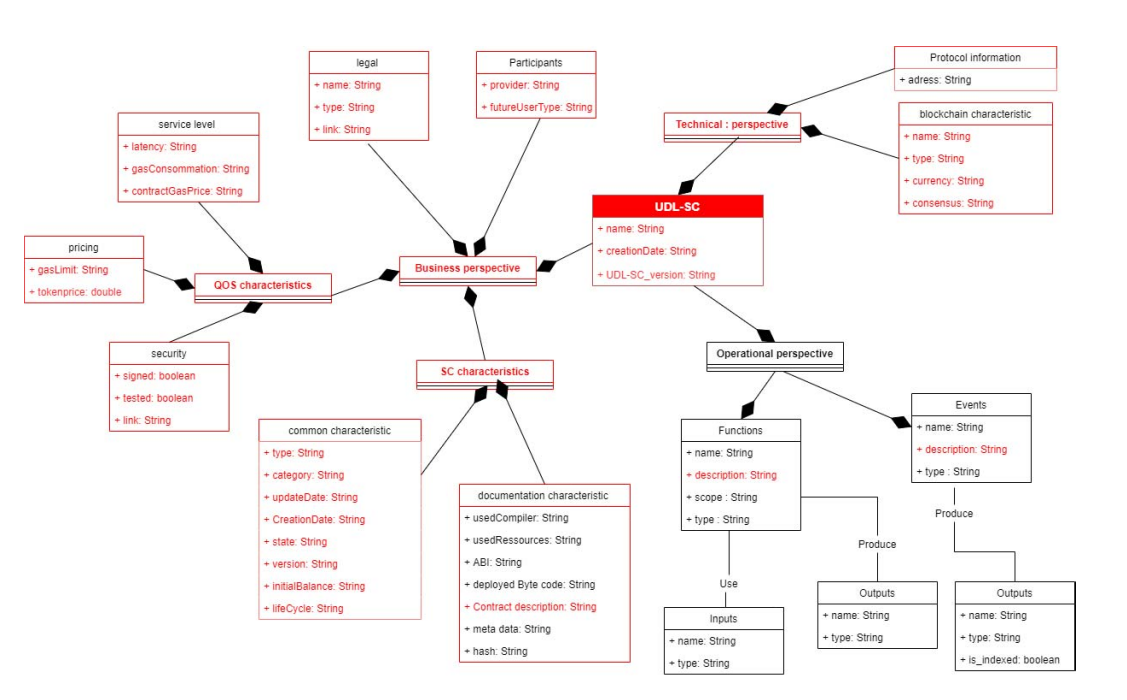
\includegraphics[width=0.7\textwidth]{resources/chapter-2/metamodel-udl-sc.png}
	\caption{Metamodel dari UDL-SC \parencite{udlsc}}
	\label{image:metamodel-udl-sc}
\end{figure}

Metamodel dari UDL-SC dapat dilihat pada Gambar \ref{image:metamodel-udl-sc}. Metamodel dari UDL-SC terdiri dari tiga perspektif utama, yaitu:

\begin{enumerate}
	\item Perspektif Operasional: Berfokus pada atribut fungsional kontrak, seperti fungsi dan event yang dapat dipanggil, beserta parameter yang terlibat.
	\item Perspektif Teknis: Berisi informasi tentang Blockchain tempat kontrak dijalankan, termasuk tipe Blockchain, konsensus, dan protokol yang digunakan.
	\item Perspektif Bisnis: meliputi karakteristik \textit{Quality of Service} (QoS) seperti konsumsi gas, harga gas, serta elemen keamanan dan legal yang terikat pada kontrak, memberikan gambaran yang lebih lengkap dan terperinci mengenai kontrak pintar secara menyeluruh.
\end{enumerate}

\begin{figure}[ht]
	\centering
	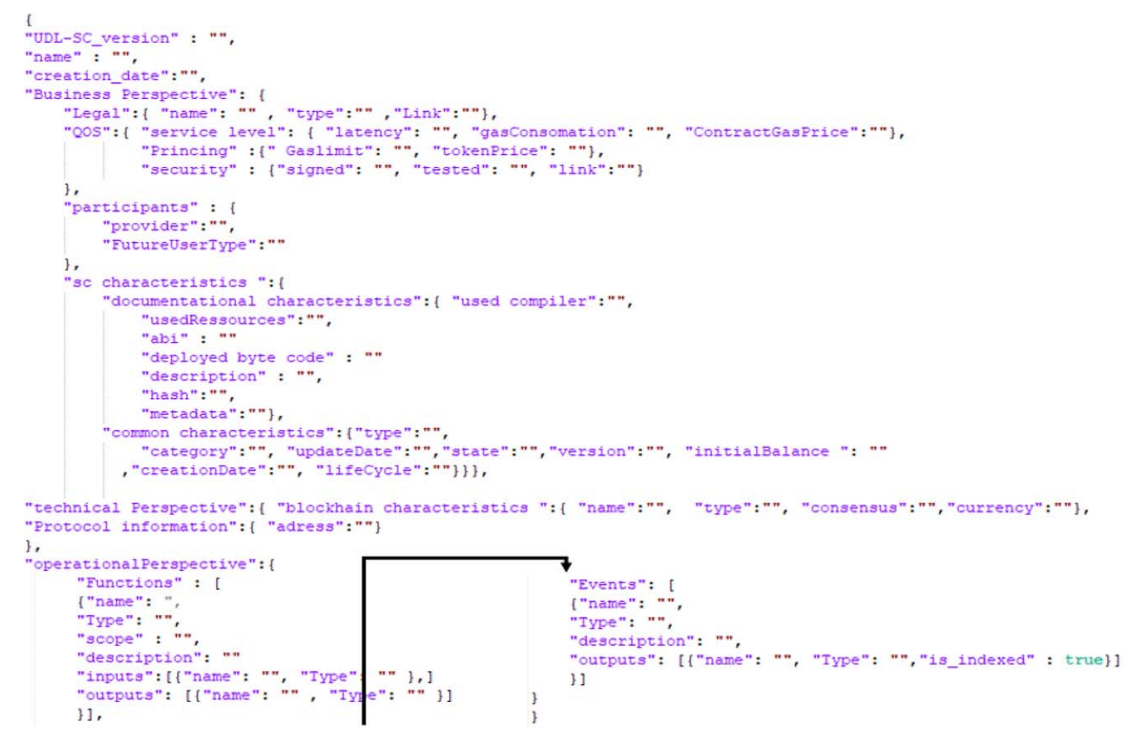
\includegraphics[width=0.7\textwidth]{resources/chapter-2/json-structure-udl-sc.png}
	\caption{Struktur deskripsi umum JSON \parencite{udlsc}}
	\label{image:json-structure-udl-sc}
\end{figure}

Gambar \ref{image:json-structure-udl-sc} menunjukkan deskripsi umum dari struktur UDL-SC dalam format JSON. Dalam penelitian ini, skema JSON dibangkitkan secara otomatis menggunakan kelas Java \texttt{SchemaGenerator}. Proses pembangkitan skema JSON ini dideskripsikan dalam gambar \ref{image:schema-generation-udl-sc}.

\begin{figure}[ht]
	\centering
	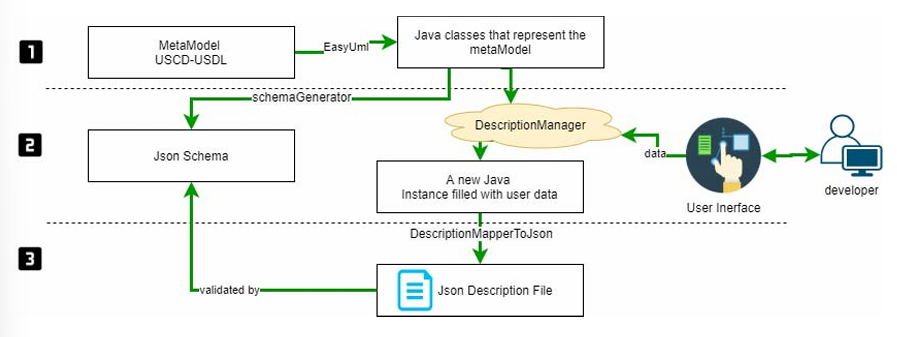
\includegraphics[width=0.7\textwidth]{resources/chapter-2/schema-generation-udl-sc.png}
	\caption{Proses pembangkitan skema JSON \parencite{udlsc}}
	\label{image:schema-generation-udl-sc}
\end{figure}

\subsection{Supporting Reuse of Smart Contracts through Service Orientation and Assisted Development}
\label{subsec:supporting-reuse-smart-contracts}

Penelitian yang dilakukan oleh \cite{guida2019supporting} membahas tantangan utama yang dihadapi pengembang saat menggunakan kembali Smart Contracts, yaitu kesulitan dalam mencari informasi yang dapat ditindaklanjuti tentang kontrak yang ada dan menulis logika integrasi untuk memanggil kontrak-kontrak yang dipilih serta mengimplementasikan fungsi yang hilang. Penelitian ini mengusulkan format deskripsi Smart Contracts yang memungkinkan pengembang untuk mencari kontrak yang tersedia secara publik, memahami fitur yang diekspos oleh kontrak tersebut, dan bagaimana cara memanggilnya dengan pendekatan berbasis layanan. Untuk mengatasi masalah integrasi, penelitian ini mengimplementasikan lingkungan pengembangan berbasis model yang terdiri dari editor pemrograman visual yang menyediakan sekumpulan konstruksi pemodelan untuk mengenkripsi pola kode yang berfokus pada penggunaan kembali Smart Contracts. Pendekatan ini diimplementasikan dan diuji pada platform Blockchain Ethereum dengan bahasa pemrograman Solidity.

\begin{figure}[ht]
	\centering
	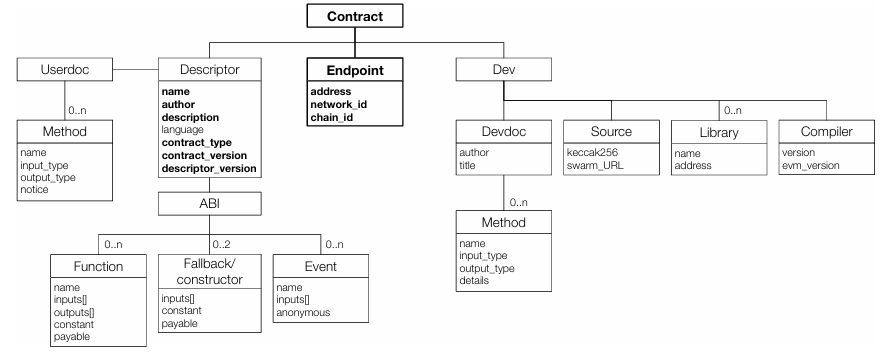
\includegraphics[width=1\textwidth]{resources/chapter-2/sc-model.png}
	\caption{Model deskripsi kontrak \parencite{guida2019supporting}}
	\label{image:sc-model}
\end{figure}

\begin{figure}[ht]
	\centering
	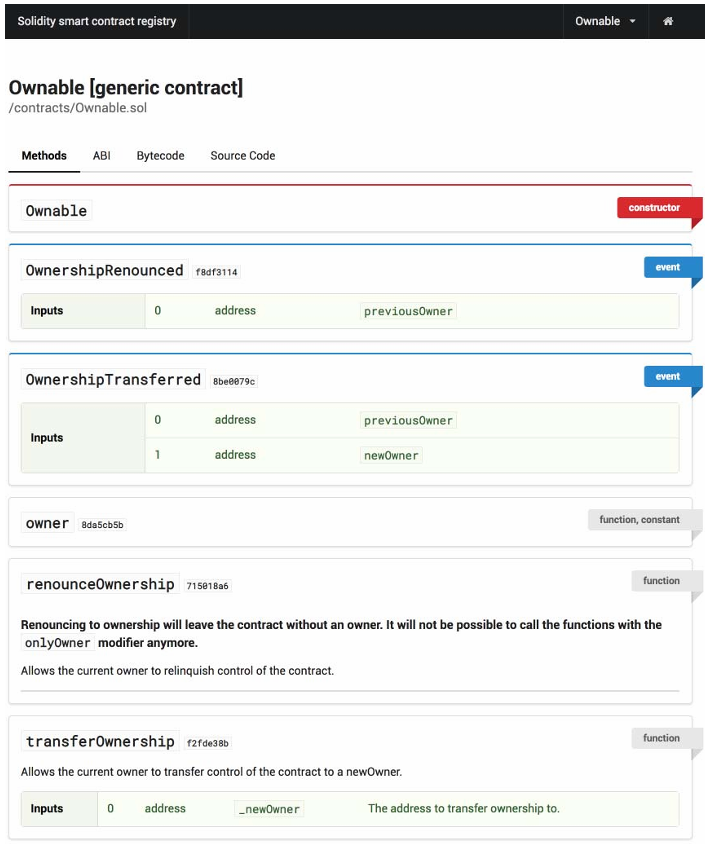
\includegraphics[width=0.7\textwidth]{resources/chapter-2/sc-registry.png}
	\caption{Tampilan Smart Contracts Registry \parencite{guida2019supporting}}
	\label{image:sc-registry}
\end{figure}

\begin{figure}[ht]
	\centering
	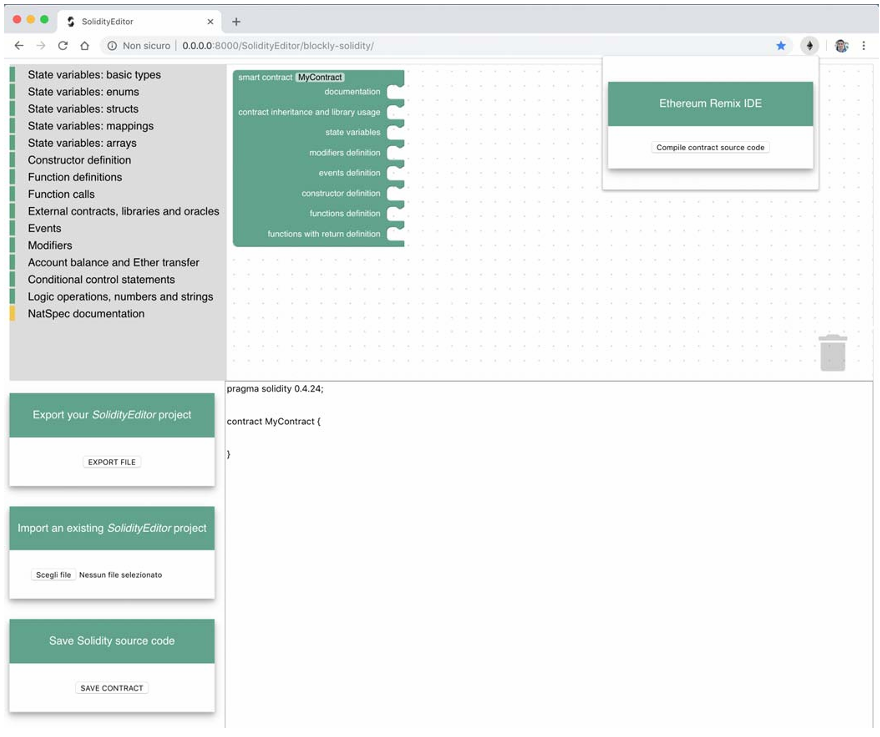
\includegraphics[width=0.7\textwidth]{resources/chapter-2/sc-editor.png}
	\caption{Tampilan Smart Contracts Visual Editor \parencite{guida2019supporting}}
	\label{image:sc-editor}
\end{figure}

\begin{figure}[ht]
	\centering
	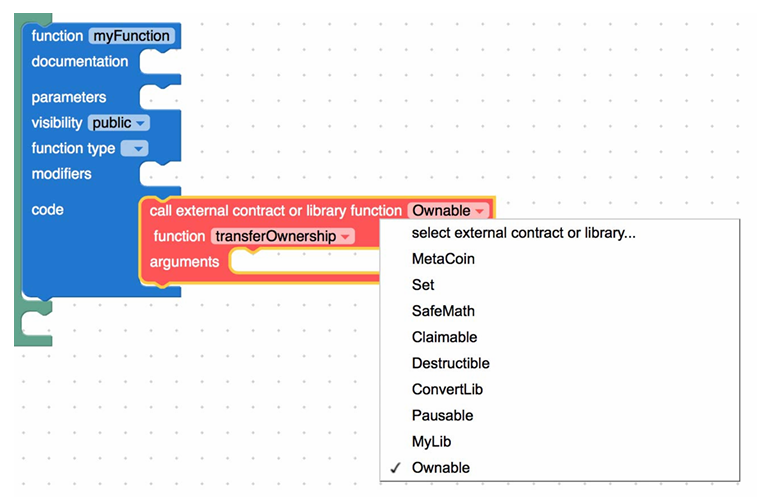
\includegraphics[width=0.7\textwidth]{resources/chapter-2/sc-editor-edit.png}
	\caption{Tampilan Smart Contract Selector \parencite{guida2019supporting}}
	\label{image:sc-editor-edit}
\end{figure}

\break

Penelitian ini menyoroti pentingnya deskripsi Smart Contracts yang memungkinkan pengembang untuk mencari dan menggunakan kontrak yang ada tanpa harus membaca kode sumbernya secara langsung. Model deskripsi kontrak yang diusulkan pada gambar \ref{image:sc-model} mencakup metadata yang sudah ada, seperti ABI dan dokumentasi, serta informasi teknis tambahan untuk memfasilitasi pencarian dan integrasi Smart Contracts. Selain itu, penelitian ini mengembangkan \textit{registry} Smart Contracts seperti yang ditunjukkan pada gambar \ref{image:sc-registry} dan \textit{editor} visual berbasis blok seperti yang ditunjukkan pada gambar \ref{image:sc-editor} dan gambar \ref{image:sc-editor-edit} untuk memudahkan pengembangan Smart Contracts yang lebih besar dan kompleks dengan cara yang lebih efisien dan dapat mengurangi kesalahan pemrograman.

\break

Implementasi ini menunjukkan bahwa penggunaan pendekatan berbasis visual, seperti \textit{editor} SolidityEditor, dapat mengurangi risiko kesalahan sintaksis, mempercepat pengembangan, dan memudahkan penggunaan kembali kode dengan mengintegrasikan pustaka kontrak eksternal seperti yang digunakan dalam studi kasus SmartTrainInsurance.

% llm with source code
% solidity summarization

% pencarian dan rekomendasi
% langchain-rag
% mm-scs


% Bab Studi Literatur digunakan untuk mendeskripsikan kajian literatur yang terkait dengan persoalan tugas akhir. Tujuan studi literatur adalah:

% \begin{enumerate}
% 	\item menunjukkan kepada pembaca adanya gap seperti pada rumusan masalah yang memang belum terselesaikan,
% 	\item memberikan pemahaman secukupnya kepada pembaca tentang teori atau pekerjaan terkait yang terkait langsung dengan penyelesaian persoalan, serta
% 	\item menyampaikan informasi apa saja yang sudah ditulis/dilaporkan oleh pihak lain (peneliti/Tugas Akhir/Tesis) tentang hasil penelitian/pekerjaan mereka yang sama atau mirip kaitannya dengan persoalan tugas akhir.
% \end{enumerate}

